% preamble not templated
\documentclass[a5paper,11pt,oneside, landscape]{article}
\usepackage[top=1cm, bottom=1cm, left=1cm, right=1cm]{geometry}
\usepackage{tikz}
\pagenumbering{gobble}
\newcommand{\s}{2.5cm}
\begin{document}

%
% repeated bingo segment (templated)
\section*{PSE BINGO}
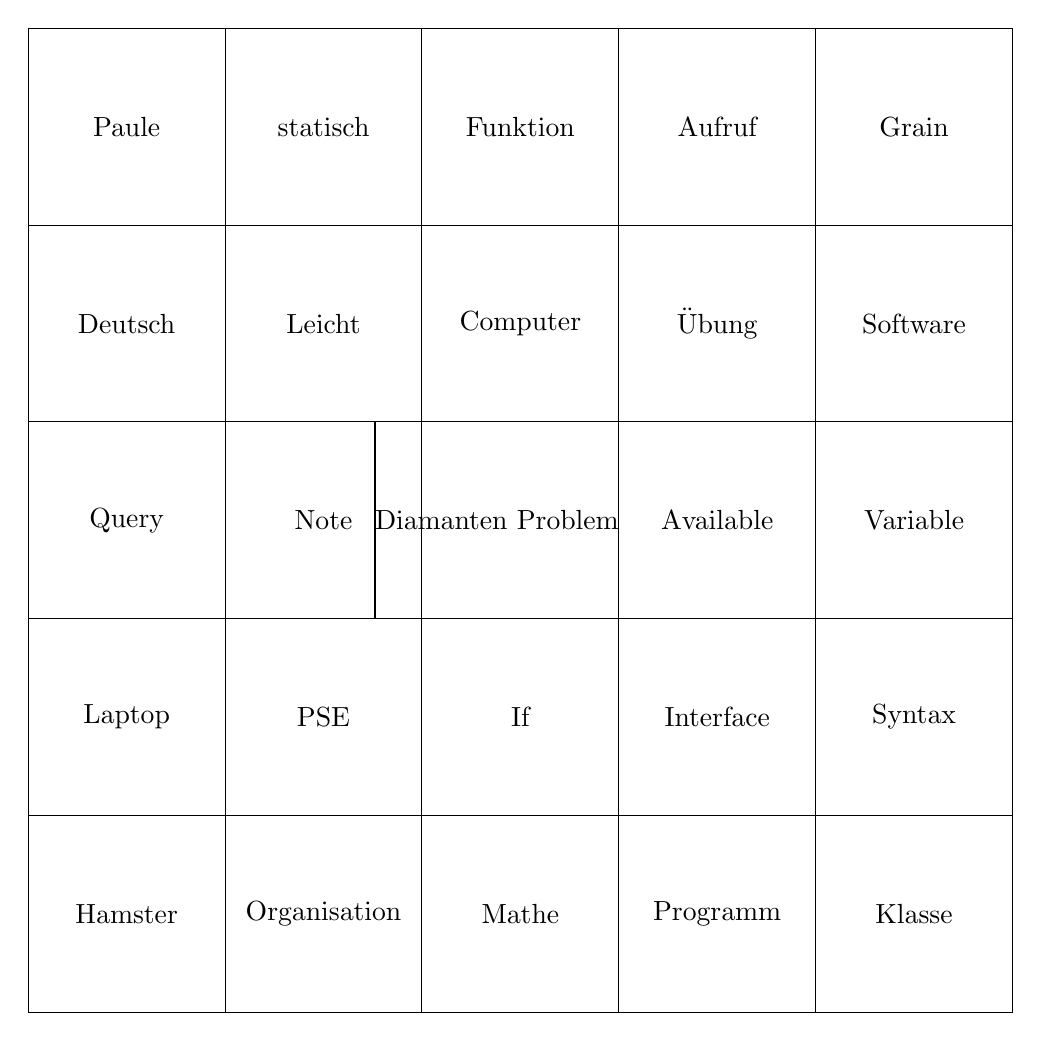
\begin{tikzpicture}[rect/.style={draw, rectangle,anchor=north east, minimum width=\s, minimum height=\s, draw, inner sep=0pt}]
    % First row
    \node[rect] (rect-1-1) at (1*\s,1*\s) {Hamster};
    \node[rect] (rect-1-2) at (2*\s,1*\s) {Organisation};
    \node[rect] (rect-1-3) at (3*\s,1*\s) {Mathe};
    \node[rect] (rect-1-4) at (4*\s,1*\s) {Programm};
    \node[rect] (rect-1-5) at (5*\s,1*\s) {Klasse};

    \node[rect] (rect-1-1) at (1*\s,2*\s) {Laptop};
    \node[rect] (rect-1-2) at (2*\s,2*\s) {PSE};
    \node[rect] (rect-1-3) at (3*\s,2*\s) {If};
    \node[rect] (rect-1-4) at (4*\s,2*\s) {Interface};
    \node[rect] (rect-1-5) at (5*\s,2*\s) {Syntax};

    \node[rect] (rect-1-1) at (1*\s,3*\s) {Query};
    \node[rect] (rect-1-2) at (2*\s,3*\s) {Note};
    \node[rect] (rect-1-3) at (3*\s,3*\s) {Diamanten Problem};
    \node[rect] (rect-1-4) at (4*\s,3*\s) {Available};
    \node[rect] (rect-1-5) at (5*\s,3*\s) {Variable};

    \node[rect] (rect-1-1) at (1*\s,4*\s) {Deutsch};
    \node[rect] (rect-1-2) at (2*\s,4*\s) {Leicht};
    \node[rect] (rect-1-3) at (3*\s,4*\s) {Computer};
    \node[rect] (rect-1-4) at (4*\s,4*\s) {Übung};
    \node[rect] (rect-1-5) at (5*\s,4*\s) {Software};

    \node[rect] (rect-1-1) at (1*\s,5*\s) {Paule};
    \node[rect] (rect-1-2) at (2*\s,5*\s) {statisch};
    \node[rect] (rect-1-3) at (3*\s,5*\s) {Funktion};
    \node[rect] (rect-1-4) at (4*\s,5*\s) {Aufruf};
    \node[rect] (rect-1-5) at (5*\s,5*\s) {Grain};

\end{tikzpicture}
\newpage
%
% repeated bingo segment (templated)
\section*{PSE BINGO}
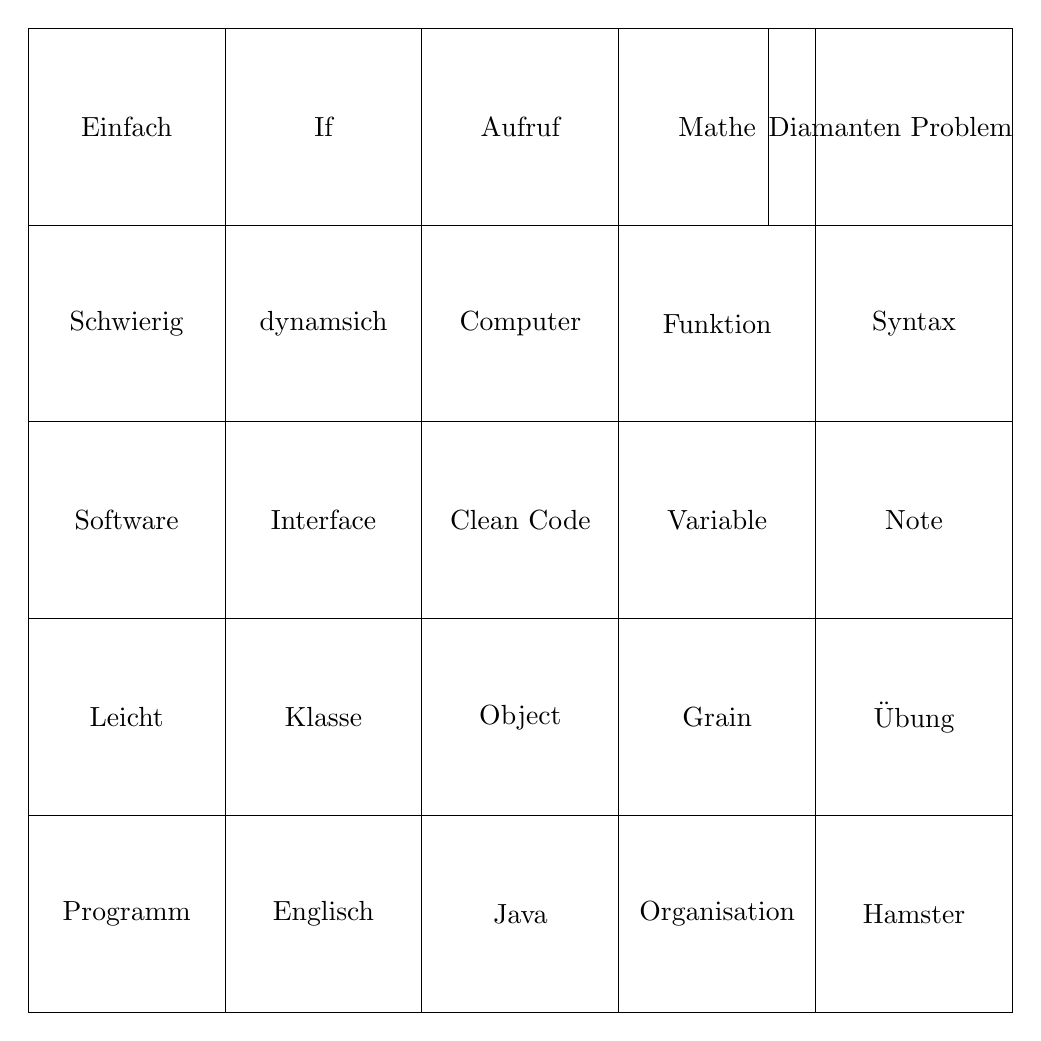
\begin{tikzpicture}[rect/.style={draw, rectangle,anchor=north east, minimum width=\s, minimum height=\s, draw, inner sep=0pt}]
    % First row
    \node[rect] (rect-1-1) at (1*\s,1*\s) {Programm};
    \node[rect] (rect-1-2) at (2*\s,1*\s) {Englisch};
    \node[rect] (rect-1-3) at (3*\s,1*\s) {Java};
    \node[rect] (rect-1-4) at (4*\s,1*\s) {Organisation};
    \node[rect] (rect-1-5) at (5*\s,1*\s) {Hamster};

    \node[rect] (rect-1-1) at (1*\s,2*\s) {Leicht};
    \node[rect] (rect-1-2) at (2*\s,2*\s) {Klasse};
    \node[rect] (rect-1-3) at (3*\s,2*\s) {Object};
    \node[rect] (rect-1-4) at (4*\s,2*\s) {Grain};
    \node[rect] (rect-1-5) at (5*\s,2*\s) {Übung};

    \node[rect] (rect-1-1) at (1*\s,3*\s) {Software};
    \node[rect] (rect-1-2) at (2*\s,3*\s) {Interface};
    \node[rect] (rect-1-3) at (3*\s,3*\s) {Clean Code};
    \node[rect] (rect-1-4) at (4*\s,3*\s) {Variable};
    \node[rect] (rect-1-5) at (5*\s,3*\s) {Note};

    \node[rect] (rect-1-1) at (1*\s,4*\s) {Schwierig};
    \node[rect] (rect-1-2) at (2*\s,4*\s) {dynamsich};
    \node[rect] (rect-1-3) at (3*\s,4*\s) {Computer};
    \node[rect] (rect-1-4) at (4*\s,4*\s) {Funktion};
    \node[rect] (rect-1-5) at (5*\s,4*\s) {Syntax};

    \node[rect] (rect-1-1) at (1*\s,5*\s) {Einfach};
    \node[rect] (rect-1-2) at (2*\s,5*\s) {If};
    \node[rect] (rect-1-3) at (3*\s,5*\s) {Aufruf};
    \node[rect] (rect-1-4) at (4*\s,5*\s) {Mathe};
    \node[rect] (rect-1-5) at (5*\s,5*\s) {Diamanten Problem};

\end{tikzpicture}
\newpage
%
% repeated bingo segment (templated)
\section*{PSE BINGO}
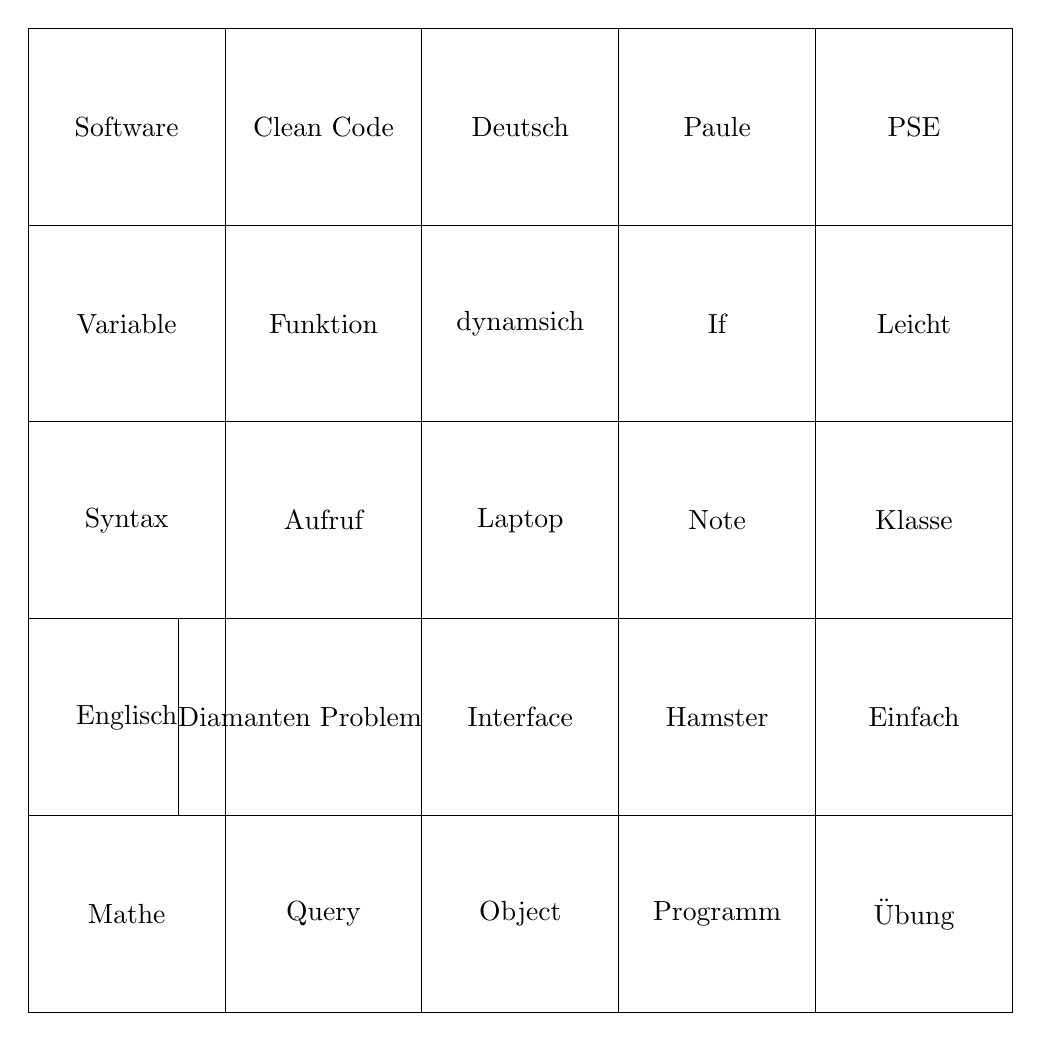
\begin{tikzpicture}[rect/.style={draw, rectangle,anchor=north east, minimum width=\s, minimum height=\s, draw, inner sep=0pt}]
    % First row
    \node[rect] (rect-1-1) at (1*\s,1*\s) {Mathe};
    \node[rect] (rect-1-2) at (2*\s,1*\s) {Query};
    \node[rect] (rect-1-3) at (3*\s,1*\s) {Object};
    \node[rect] (rect-1-4) at (4*\s,1*\s) {Programm};
    \node[rect] (rect-1-5) at (5*\s,1*\s) {Übung};

    \node[rect] (rect-1-1) at (1*\s,2*\s) {Englisch};
    \node[rect] (rect-1-2) at (2*\s,2*\s) {Diamanten Problem};
    \node[rect] (rect-1-3) at (3*\s,2*\s) {Interface};
    \node[rect] (rect-1-4) at (4*\s,2*\s) {Hamster};
    \node[rect] (rect-1-5) at (5*\s,2*\s) {Einfach};

    \node[rect] (rect-1-1) at (1*\s,3*\s) {Syntax};
    \node[rect] (rect-1-2) at (2*\s,3*\s) {Aufruf};
    \node[rect] (rect-1-3) at (3*\s,3*\s) {Laptop};
    \node[rect] (rect-1-4) at (4*\s,3*\s) {Note};
    \node[rect] (rect-1-5) at (5*\s,3*\s) {Klasse};

    \node[rect] (rect-1-1) at (1*\s,4*\s) {Variable};
    \node[rect] (rect-1-2) at (2*\s,4*\s) {Funktion};
    \node[rect] (rect-1-3) at (3*\s,4*\s) {dynamsich};
    \node[rect] (rect-1-4) at (4*\s,4*\s) {If};
    \node[rect] (rect-1-5) at (5*\s,4*\s) {Leicht};

    \node[rect] (rect-1-1) at (1*\s,5*\s) {Software};
    \node[rect] (rect-1-2) at (2*\s,5*\s) {Clean Code};
    \node[rect] (rect-1-3) at (3*\s,5*\s) {Deutsch};
    \node[rect] (rect-1-4) at (4*\s,5*\s) {Paule};
    \node[rect] (rect-1-5) at (5*\s,5*\s) {PSE};

\end{tikzpicture}
\newpage
%
% repeated bingo segment (templated)
\section*{PSE BINGO}
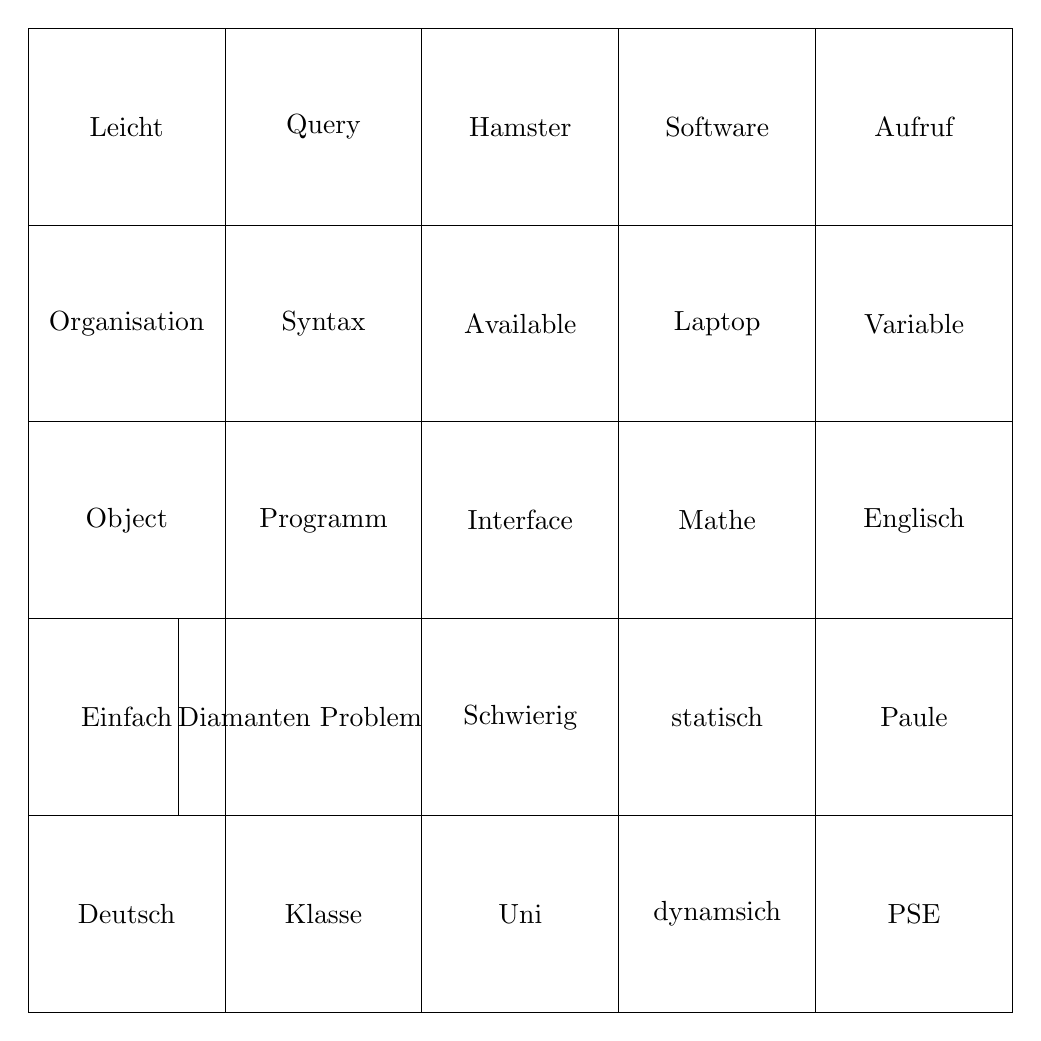
\begin{tikzpicture}[rect/.style={draw, rectangle,anchor=north east, minimum width=\s, minimum height=\s, draw, inner sep=0pt}]
    % First row
    \node[rect] (rect-1-1) at (1*\s,1*\s) {Deutsch};
    \node[rect] (rect-1-2) at (2*\s,1*\s) {Klasse};
    \node[rect] (rect-1-3) at (3*\s,1*\s) {Uni};
    \node[rect] (rect-1-4) at (4*\s,1*\s) {dynamsich};
    \node[rect] (rect-1-5) at (5*\s,1*\s) {PSE};

    \node[rect] (rect-1-1) at (1*\s,2*\s) {Einfach};
    \node[rect] (rect-1-2) at (2*\s,2*\s) {Diamanten Problem};
    \node[rect] (rect-1-3) at (3*\s,2*\s) {Schwierig};
    \node[rect] (rect-1-4) at (4*\s,2*\s) {statisch};
    \node[rect] (rect-1-5) at (5*\s,2*\s) {Paule};

    \node[rect] (rect-1-1) at (1*\s,3*\s) {Object};
    \node[rect] (rect-1-2) at (2*\s,3*\s) {Programm};
    \node[rect] (rect-1-3) at (3*\s,3*\s) {Interface};
    \node[rect] (rect-1-4) at (4*\s,3*\s) {Mathe};
    \node[rect] (rect-1-5) at (5*\s,3*\s) {Englisch};

    \node[rect] (rect-1-1) at (1*\s,4*\s) {Organisation};
    \node[rect] (rect-1-2) at (2*\s,4*\s) {Syntax};
    \node[rect] (rect-1-3) at (3*\s,4*\s) {Available};
    \node[rect] (rect-1-4) at (4*\s,4*\s) {Laptop};
    \node[rect] (rect-1-5) at (5*\s,4*\s) {Variable};

    \node[rect] (rect-1-1) at (1*\s,5*\s) {Leicht};
    \node[rect] (rect-1-2) at (2*\s,5*\s) {Query};
    \node[rect] (rect-1-3) at (3*\s,5*\s) {Hamster};
    \node[rect] (rect-1-4) at (4*\s,5*\s) {Software};
    \node[rect] (rect-1-5) at (5*\s,5*\s) {Aufruf};

\end{tikzpicture}
\newpage
%
% repeated bingo segment (templated)
\section*{PSE BINGO}
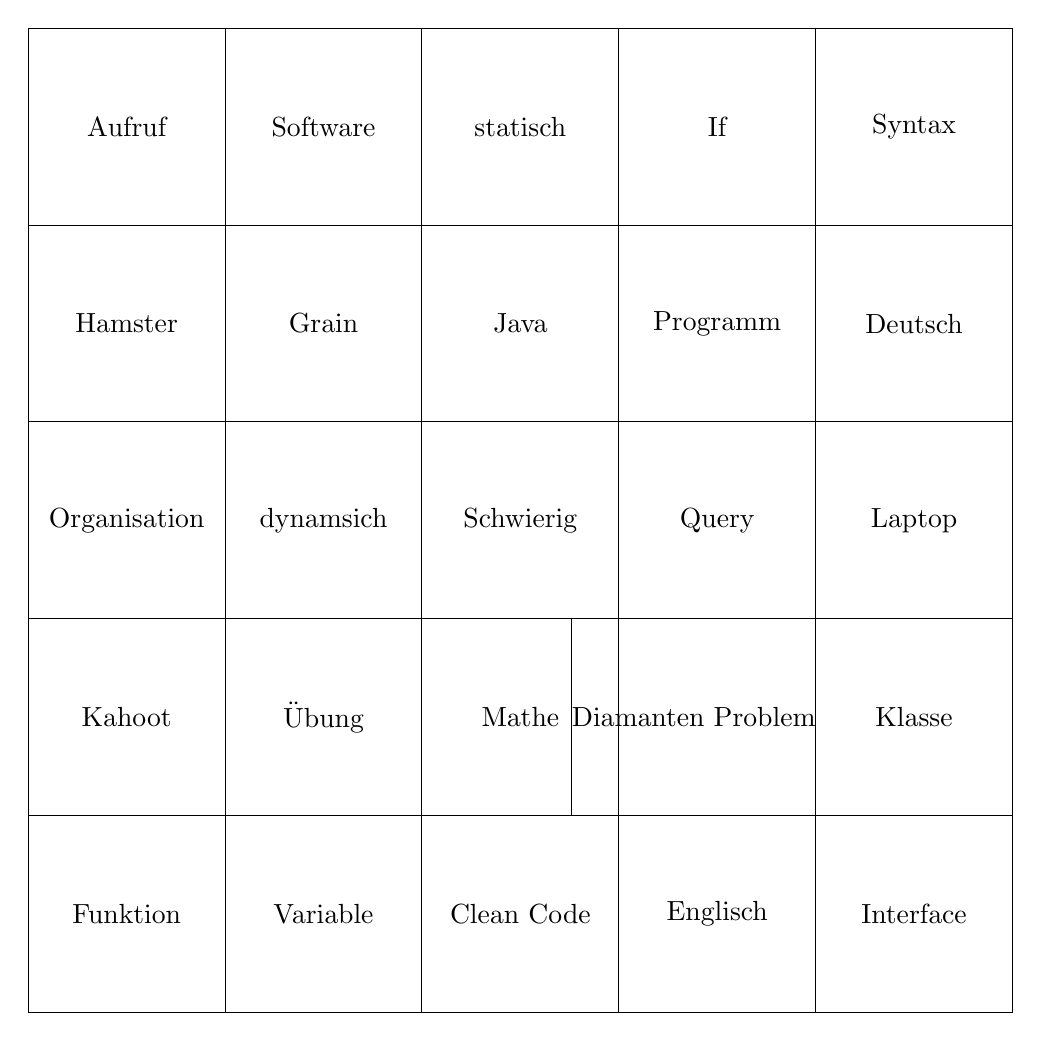
\begin{tikzpicture}[rect/.style={draw, rectangle,anchor=north east, minimum width=\s, minimum height=\s, draw, inner sep=0pt}]
    % First row
    \node[rect] (rect-1-1) at (1*\s,1*\s) {Funktion};
    \node[rect] (rect-1-2) at (2*\s,1*\s) {Variable};
    \node[rect] (rect-1-3) at (3*\s,1*\s) {Clean Code};
    \node[rect] (rect-1-4) at (4*\s,1*\s) {Englisch};
    \node[rect] (rect-1-5) at (5*\s,1*\s) {Interface};

    \node[rect] (rect-1-1) at (1*\s,2*\s) {Kahoot};
    \node[rect] (rect-1-2) at (2*\s,2*\s) {Übung};
    \node[rect] (rect-1-3) at (3*\s,2*\s) {Mathe};
    \node[rect] (rect-1-4) at (4*\s,2*\s) {Diamanten Problem};
    \node[rect] (rect-1-5) at (5*\s,2*\s) {Klasse};

    \node[rect] (rect-1-1) at (1*\s,3*\s) {Organisation};
    \node[rect] (rect-1-2) at (2*\s,3*\s) {dynamsich};
    \node[rect] (rect-1-3) at (3*\s,3*\s) {Schwierig};
    \node[rect] (rect-1-4) at (4*\s,3*\s) {Query};
    \node[rect] (rect-1-5) at (5*\s,3*\s) {Laptop};

    \node[rect] (rect-1-1) at (1*\s,4*\s) {Hamster};
    \node[rect] (rect-1-2) at (2*\s,4*\s) {Grain};
    \node[rect] (rect-1-3) at (3*\s,4*\s) {Java};
    \node[rect] (rect-1-4) at (4*\s,4*\s) {Programm};
    \node[rect] (rect-1-5) at (5*\s,4*\s) {Deutsch};

    \node[rect] (rect-1-1) at (1*\s,5*\s) {Aufruf};
    \node[rect] (rect-1-2) at (2*\s,5*\s) {Software};
    \node[rect] (rect-1-3) at (3*\s,5*\s) {statisch};
    \node[rect] (rect-1-4) at (4*\s,5*\s) {If};
    \node[rect] (rect-1-5) at (5*\s,5*\s) {Syntax};

\end{tikzpicture}
\newpage
%
% repeated bingo segment (templated)
\section*{PSE BINGO}
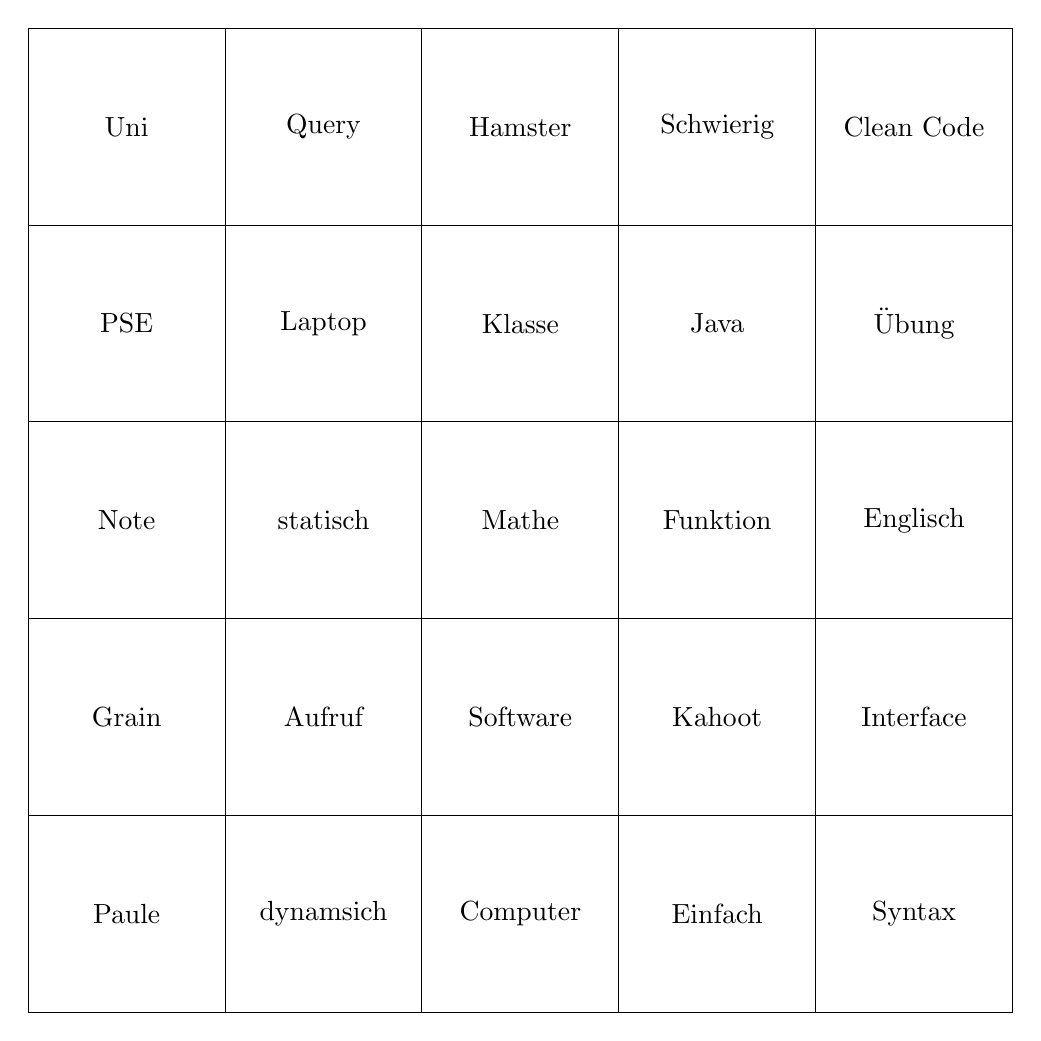
\begin{tikzpicture}[rect/.style={draw, rectangle,anchor=north east, minimum width=\s, minimum height=\s, draw, inner sep=0pt}]
    % First row
    \node[rect] (rect-1-1) at (1*\s,1*\s) {Paule};
    \node[rect] (rect-1-2) at (2*\s,1*\s) {dynamsich};
    \node[rect] (rect-1-3) at (3*\s,1*\s) {Computer};
    \node[rect] (rect-1-4) at (4*\s,1*\s) {Einfach};
    \node[rect] (rect-1-5) at (5*\s,1*\s) {Syntax};

    \node[rect] (rect-1-1) at (1*\s,2*\s) {Grain};
    \node[rect] (rect-1-2) at (2*\s,2*\s) {Aufruf};
    \node[rect] (rect-1-3) at (3*\s,2*\s) {Software};
    \node[rect] (rect-1-4) at (4*\s,2*\s) {Kahoot};
    \node[rect] (rect-1-5) at (5*\s,2*\s) {Interface};

    \node[rect] (rect-1-1) at (1*\s,3*\s) {Note};
    \node[rect] (rect-1-2) at (2*\s,3*\s) {statisch};
    \node[rect] (rect-1-3) at (3*\s,3*\s) {Mathe};
    \node[rect] (rect-1-4) at (4*\s,3*\s) {Funktion};
    \node[rect] (rect-1-5) at (5*\s,3*\s) {Englisch};

    \node[rect] (rect-1-1) at (1*\s,4*\s) {PSE};
    \node[rect] (rect-1-2) at (2*\s,4*\s) {Laptop};
    \node[rect] (rect-1-3) at (3*\s,4*\s) {Klasse};
    \node[rect] (rect-1-4) at (4*\s,4*\s) {Java};
    \node[rect] (rect-1-5) at (5*\s,4*\s) {Übung};

    \node[rect] (rect-1-1) at (1*\s,5*\s) {Uni};
    \node[rect] (rect-1-2) at (2*\s,5*\s) {Query};
    \node[rect] (rect-1-3) at (3*\s,5*\s) {Hamster};
    \node[rect] (rect-1-4) at (4*\s,5*\s) {Schwierig};
    \node[rect] (rect-1-5) at (5*\s,5*\s) {Clean Code};

\end{tikzpicture}
\newpage
%
% repeated bingo segment (templated)
\section*{PSE BINGO}
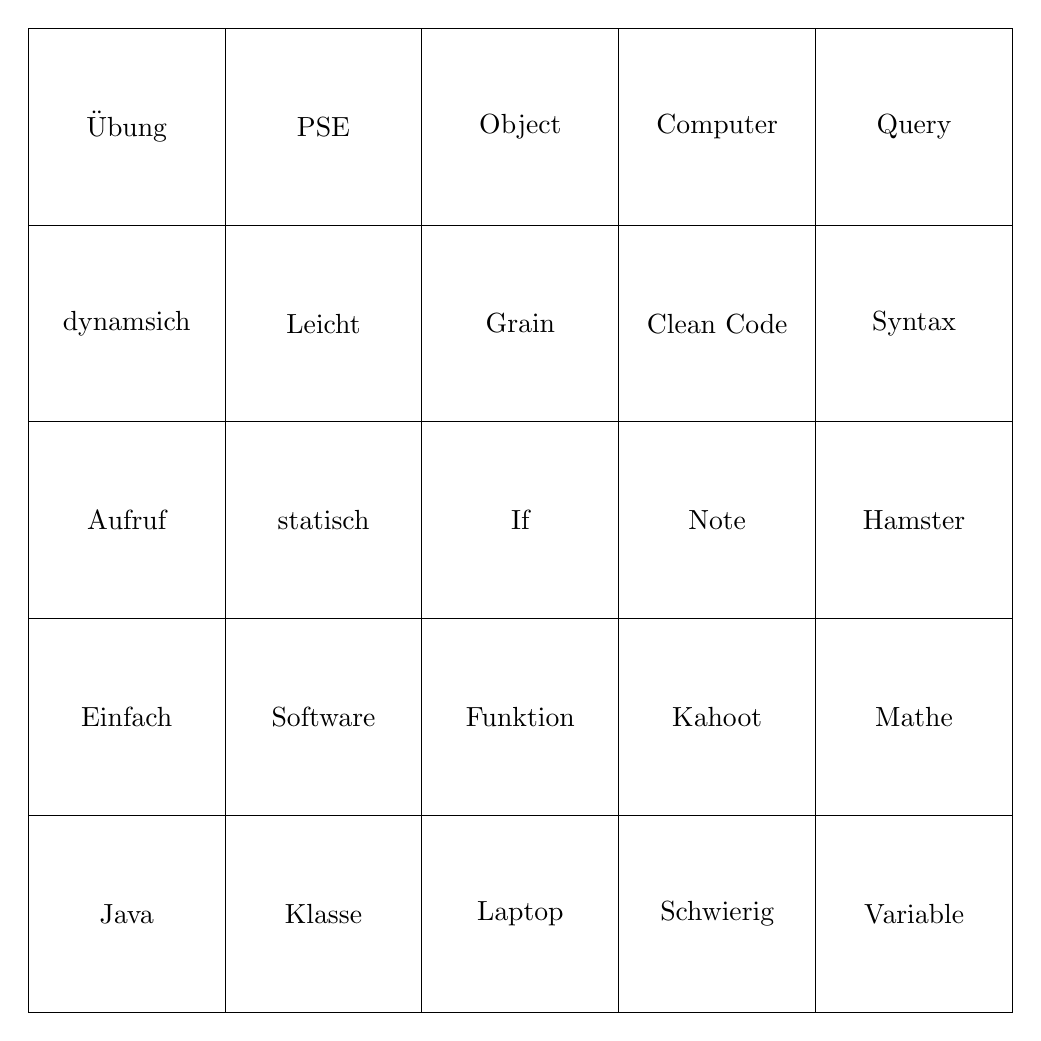
\begin{tikzpicture}[rect/.style={draw, rectangle,anchor=north east, minimum width=\s, minimum height=\s, draw, inner sep=0pt}]
    % First row
    \node[rect] (rect-1-1) at (1*\s,1*\s) {Java};
    \node[rect] (rect-1-2) at (2*\s,1*\s) {Klasse};
    \node[rect] (rect-1-3) at (3*\s,1*\s) {Laptop};
    \node[rect] (rect-1-4) at (4*\s,1*\s) {Schwierig};
    \node[rect] (rect-1-5) at (5*\s,1*\s) {Variable};

    \node[rect] (rect-1-1) at (1*\s,2*\s) {Einfach};
    \node[rect] (rect-1-2) at (2*\s,2*\s) {Software};
    \node[rect] (rect-1-3) at (3*\s,2*\s) {Funktion};
    \node[rect] (rect-1-4) at (4*\s,2*\s) {Kahoot};
    \node[rect] (rect-1-5) at (5*\s,2*\s) {Mathe};

    \node[rect] (rect-1-1) at (1*\s,3*\s) {Aufruf};
    \node[rect] (rect-1-2) at (2*\s,3*\s) {statisch};
    \node[rect] (rect-1-3) at (3*\s,3*\s) {If};
    \node[rect] (rect-1-4) at (4*\s,3*\s) {Note};
    \node[rect] (rect-1-5) at (5*\s,3*\s) {Hamster};

    \node[rect] (rect-1-1) at (1*\s,4*\s) {dynamsich};
    \node[rect] (rect-1-2) at (2*\s,4*\s) {Leicht};
    \node[rect] (rect-1-3) at (3*\s,4*\s) {Grain};
    \node[rect] (rect-1-4) at (4*\s,4*\s) {Clean Code};
    \node[rect] (rect-1-5) at (5*\s,4*\s) {Syntax};

    \node[rect] (rect-1-1) at (1*\s,5*\s) {Übung};
    \node[rect] (rect-1-2) at (2*\s,5*\s) {PSE};
    \node[rect] (rect-1-3) at (3*\s,5*\s) {Object};
    \node[rect] (rect-1-4) at (4*\s,5*\s) {Computer};
    \node[rect] (rect-1-5) at (5*\s,5*\s) {Query};

\end{tikzpicture}
\newpage
%
% repeated bingo segment (templated)
\section*{PSE BINGO}
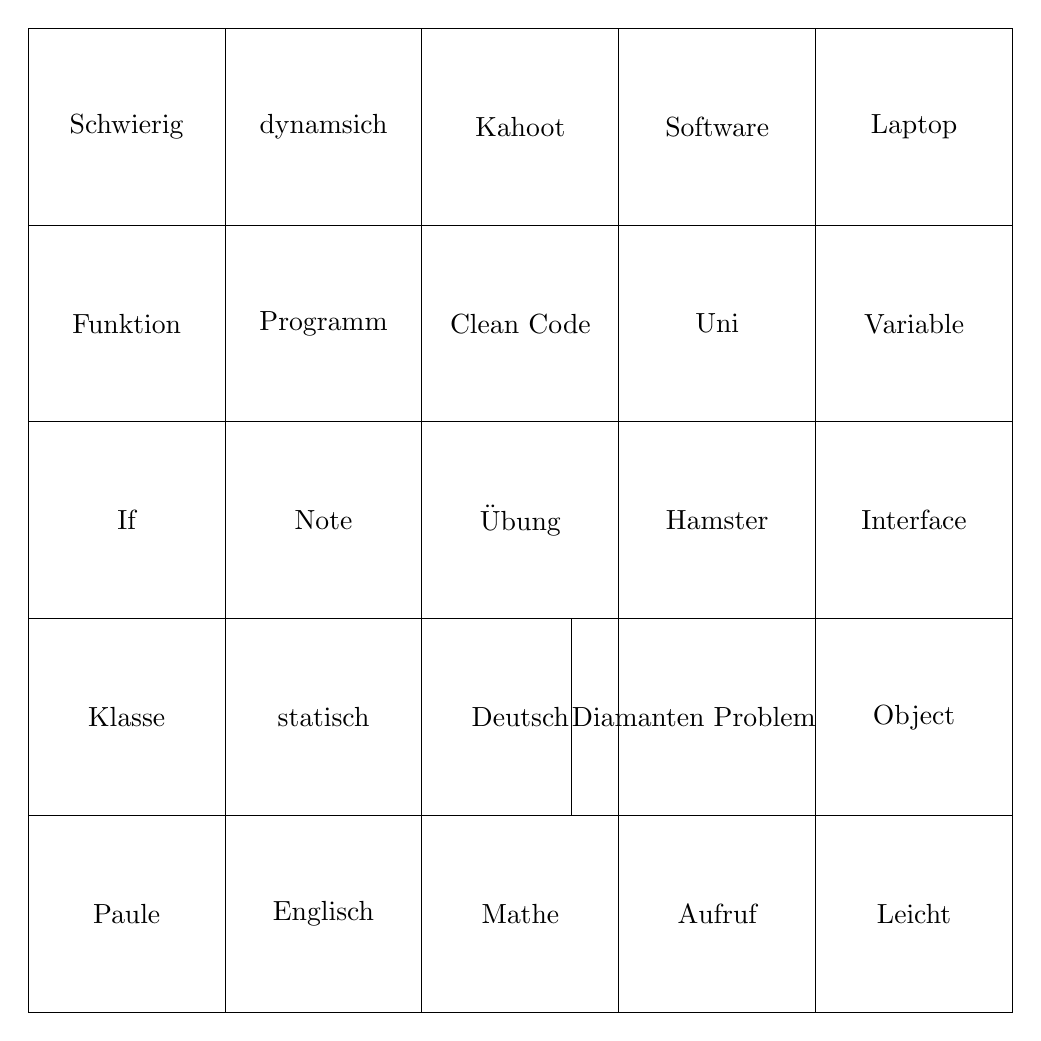
\begin{tikzpicture}[rect/.style={draw, rectangle,anchor=north east, minimum width=\s, minimum height=\s, draw, inner sep=0pt}]
    % First row
    \node[rect] (rect-1-1) at (1*\s,1*\s) {Paule};
    \node[rect] (rect-1-2) at (2*\s,1*\s) {Englisch};
    \node[rect] (rect-1-3) at (3*\s,1*\s) {Mathe};
    \node[rect] (rect-1-4) at (4*\s,1*\s) {Aufruf};
    \node[rect] (rect-1-5) at (5*\s,1*\s) {Leicht};

    \node[rect] (rect-1-1) at (1*\s,2*\s) {Klasse};
    \node[rect] (rect-1-2) at (2*\s,2*\s) {statisch};
    \node[rect] (rect-1-3) at (3*\s,2*\s) {Deutsch};
    \node[rect] (rect-1-4) at (4*\s,2*\s) {Diamanten Problem};
    \node[rect] (rect-1-5) at (5*\s,2*\s) {Object};

    \node[rect] (rect-1-1) at (1*\s,3*\s) {If};
    \node[rect] (rect-1-2) at (2*\s,3*\s) {Note};
    \node[rect] (rect-1-3) at (3*\s,3*\s) {Übung};
    \node[rect] (rect-1-4) at (4*\s,3*\s) {Hamster};
    \node[rect] (rect-1-5) at (5*\s,3*\s) {Interface};

    \node[rect] (rect-1-1) at (1*\s,4*\s) {Funktion};
    \node[rect] (rect-1-2) at (2*\s,4*\s) {Programm};
    \node[rect] (rect-1-3) at (3*\s,4*\s) {Clean Code};
    \node[rect] (rect-1-4) at (4*\s,4*\s) {Uni};
    \node[rect] (rect-1-5) at (5*\s,4*\s) {Variable};

    \node[rect] (rect-1-1) at (1*\s,5*\s) {Schwierig};
    \node[rect] (rect-1-2) at (2*\s,5*\s) {dynamsich};
    \node[rect] (rect-1-3) at (3*\s,5*\s) {Kahoot};
    \node[rect] (rect-1-4) at (4*\s,5*\s) {Software};
    \node[rect] (rect-1-5) at (5*\s,5*\s) {Laptop};

\end{tikzpicture}
\newpage
%
% repeated bingo segment (templated)
\section*{PSE BINGO}
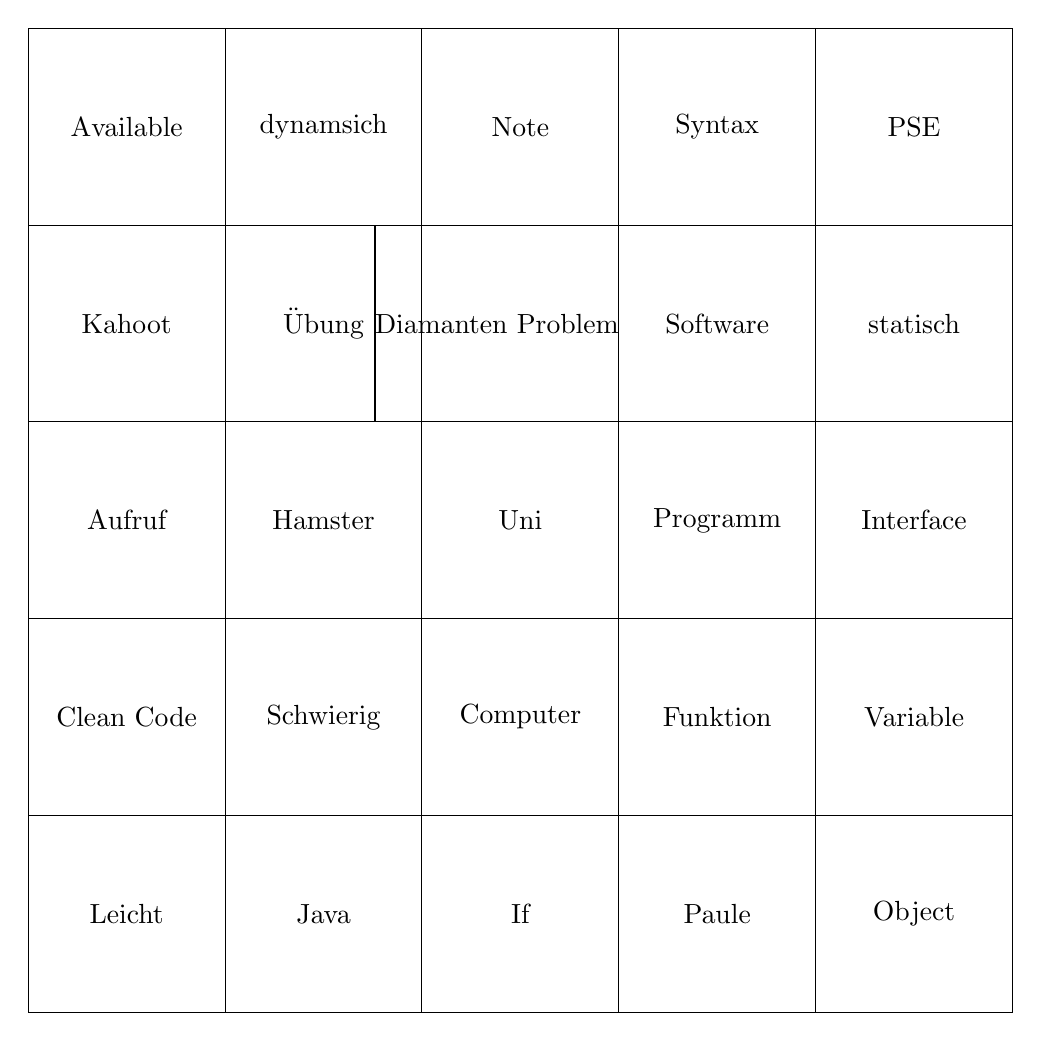
\begin{tikzpicture}[rect/.style={draw, rectangle,anchor=north east, minimum width=\s, minimum height=\s, draw, inner sep=0pt}]
    % First row
    \node[rect] (rect-1-1) at (1*\s,1*\s) {Leicht};
    \node[rect] (rect-1-2) at (2*\s,1*\s) {Java};
    \node[rect] (rect-1-3) at (3*\s,1*\s) {If};
    \node[rect] (rect-1-4) at (4*\s,1*\s) {Paule};
    \node[rect] (rect-1-5) at (5*\s,1*\s) {Object};

    \node[rect] (rect-1-1) at (1*\s,2*\s) {Clean Code};
    \node[rect] (rect-1-2) at (2*\s,2*\s) {Schwierig};
    \node[rect] (rect-1-3) at (3*\s,2*\s) {Computer};
    \node[rect] (rect-1-4) at (4*\s,2*\s) {Funktion};
    \node[rect] (rect-1-5) at (5*\s,2*\s) {Variable};

    \node[rect] (rect-1-1) at (1*\s,3*\s) {Aufruf};
    \node[rect] (rect-1-2) at (2*\s,3*\s) {Hamster};
    \node[rect] (rect-1-3) at (3*\s,3*\s) {Uni};
    \node[rect] (rect-1-4) at (4*\s,3*\s) {Programm};
    \node[rect] (rect-1-5) at (5*\s,3*\s) {Interface};

    \node[rect] (rect-1-1) at (1*\s,4*\s) {Kahoot};
    \node[rect] (rect-1-2) at (2*\s,4*\s) {Übung};
    \node[rect] (rect-1-3) at (3*\s,4*\s) {Diamanten Problem};
    \node[rect] (rect-1-4) at (4*\s,4*\s) {Software};
    \node[rect] (rect-1-5) at (5*\s,4*\s) {statisch};

    \node[rect] (rect-1-1) at (1*\s,5*\s) {Available};
    \node[rect] (rect-1-2) at (2*\s,5*\s) {dynamsich};
    \node[rect] (rect-1-3) at (3*\s,5*\s) {Note};
    \node[rect] (rect-1-4) at (4*\s,5*\s) {Syntax};
    \node[rect] (rect-1-5) at (5*\s,5*\s) {PSE};

\end{tikzpicture}
\newpage
%
% repeated bingo segment (templated)
\section*{PSE BINGO}
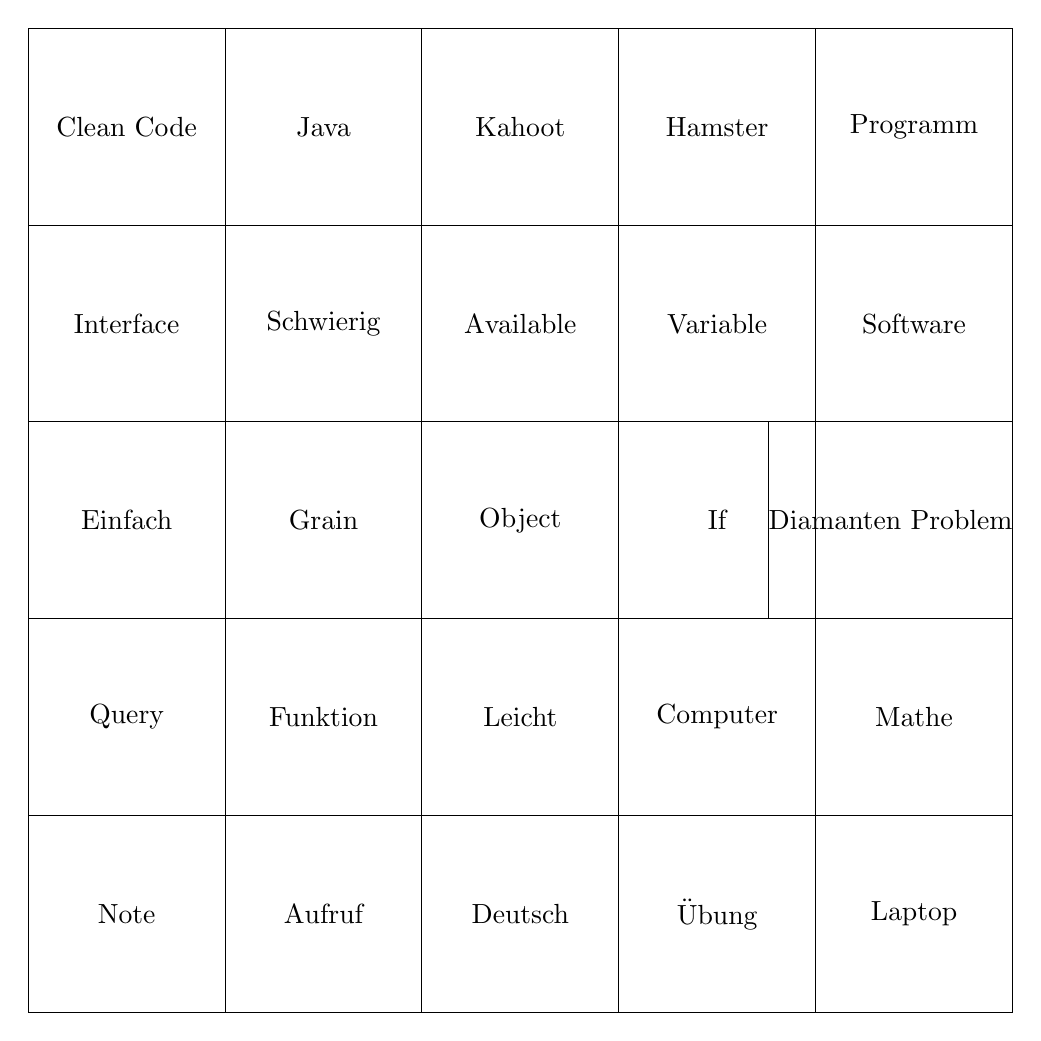
\begin{tikzpicture}[rect/.style={draw, rectangle,anchor=north east, minimum width=\s, minimum height=\s, draw, inner sep=0pt}]
    % First row
    \node[rect] (rect-1-1) at (1*\s,1*\s) {Note};
    \node[rect] (rect-1-2) at (2*\s,1*\s) {Aufruf};
    \node[rect] (rect-1-3) at (3*\s,1*\s) {Deutsch};
    \node[rect] (rect-1-4) at (4*\s,1*\s) {Übung};
    \node[rect] (rect-1-5) at (5*\s,1*\s) {Laptop};

    \node[rect] (rect-1-1) at (1*\s,2*\s) {Query};
    \node[rect] (rect-1-2) at (2*\s,2*\s) {Funktion};
    \node[rect] (rect-1-3) at (3*\s,2*\s) {Leicht};
    \node[rect] (rect-1-4) at (4*\s,2*\s) {Computer};
    \node[rect] (rect-1-5) at (5*\s,2*\s) {Mathe};

    \node[rect] (rect-1-1) at (1*\s,3*\s) {Einfach};
    \node[rect] (rect-1-2) at (2*\s,3*\s) {Grain};
    \node[rect] (rect-1-3) at (3*\s,3*\s) {Object};
    \node[rect] (rect-1-4) at (4*\s,3*\s) {If};
    \node[rect] (rect-1-5) at (5*\s,3*\s) {Diamanten Problem};

    \node[rect] (rect-1-1) at (1*\s,4*\s) {Interface};
    \node[rect] (rect-1-2) at (2*\s,4*\s) {Schwierig};
    \node[rect] (rect-1-3) at (3*\s,4*\s) {Available};
    \node[rect] (rect-1-4) at (4*\s,4*\s) {Variable};
    \node[rect] (rect-1-5) at (5*\s,4*\s) {Software};

    \node[rect] (rect-1-1) at (1*\s,5*\s) {Clean Code};
    \node[rect] (rect-1-2) at (2*\s,5*\s) {Java};
    \node[rect] (rect-1-3) at (3*\s,5*\s) {Kahoot};
    \node[rect] (rect-1-4) at (4*\s,5*\s) {Hamster};
    \node[rect] (rect-1-5) at (5*\s,5*\s) {Programm};

\end{tikzpicture}
\newpage
%
% repeated bingo segment (templated)
\section*{PSE BINGO}
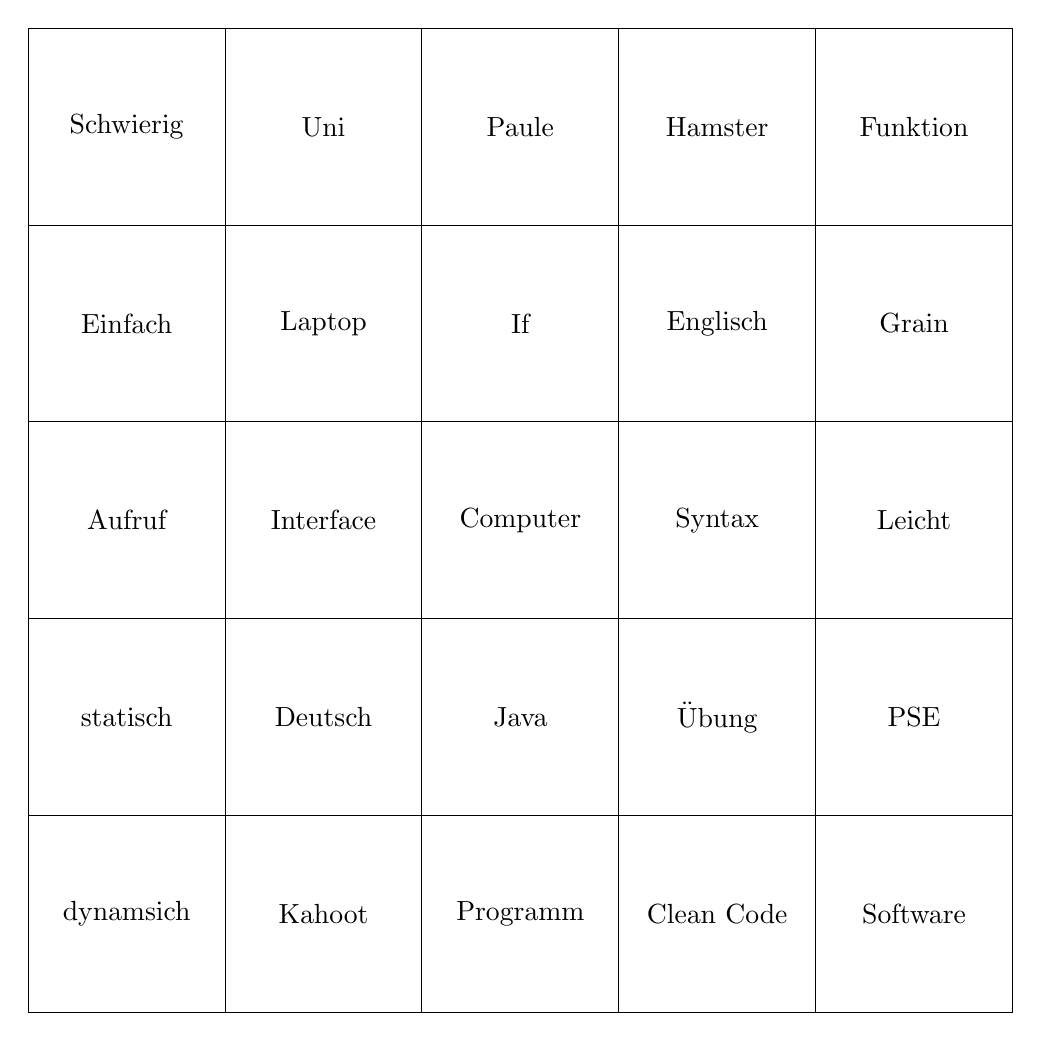
\begin{tikzpicture}[rect/.style={draw, rectangle,anchor=north east, minimum width=\s, minimum height=\s, draw, inner sep=0pt}]
    % First row
    \node[rect] (rect-1-1) at (1*\s,1*\s) {dynamsich};
    \node[rect] (rect-1-2) at (2*\s,1*\s) {Kahoot};
    \node[rect] (rect-1-3) at (3*\s,1*\s) {Programm};
    \node[rect] (rect-1-4) at (4*\s,1*\s) {Clean Code};
    \node[rect] (rect-1-5) at (5*\s,1*\s) {Software};

    \node[rect] (rect-1-1) at (1*\s,2*\s) {statisch};
    \node[rect] (rect-1-2) at (2*\s,2*\s) {Deutsch};
    \node[rect] (rect-1-3) at (3*\s,2*\s) {Java};
    \node[rect] (rect-1-4) at (4*\s,2*\s) {Übung};
    \node[rect] (rect-1-5) at (5*\s,2*\s) {PSE};

    \node[rect] (rect-1-1) at (1*\s,3*\s) {Aufruf};
    \node[rect] (rect-1-2) at (2*\s,3*\s) {Interface};
    \node[rect] (rect-1-3) at (3*\s,3*\s) {Computer};
    \node[rect] (rect-1-4) at (4*\s,3*\s) {Syntax};
    \node[rect] (rect-1-5) at (5*\s,3*\s) {Leicht};

    \node[rect] (rect-1-1) at (1*\s,4*\s) {Einfach};
    \node[rect] (rect-1-2) at (2*\s,4*\s) {Laptop};
    \node[rect] (rect-1-3) at (3*\s,4*\s) {If};
    \node[rect] (rect-1-4) at (4*\s,4*\s) {Englisch};
    \node[rect] (rect-1-5) at (5*\s,4*\s) {Grain};

    \node[rect] (rect-1-1) at (1*\s,5*\s) {Schwierig};
    \node[rect] (rect-1-2) at (2*\s,5*\s) {Uni};
    \node[rect] (rect-1-3) at (3*\s,5*\s) {Paule};
    \node[rect] (rect-1-4) at (4*\s,5*\s) {Hamster};
    \node[rect] (rect-1-5) at (5*\s,5*\s) {Funktion};

\end{tikzpicture}
\newpage
%
% repeated bingo segment (templated)
\section*{PSE BINGO}
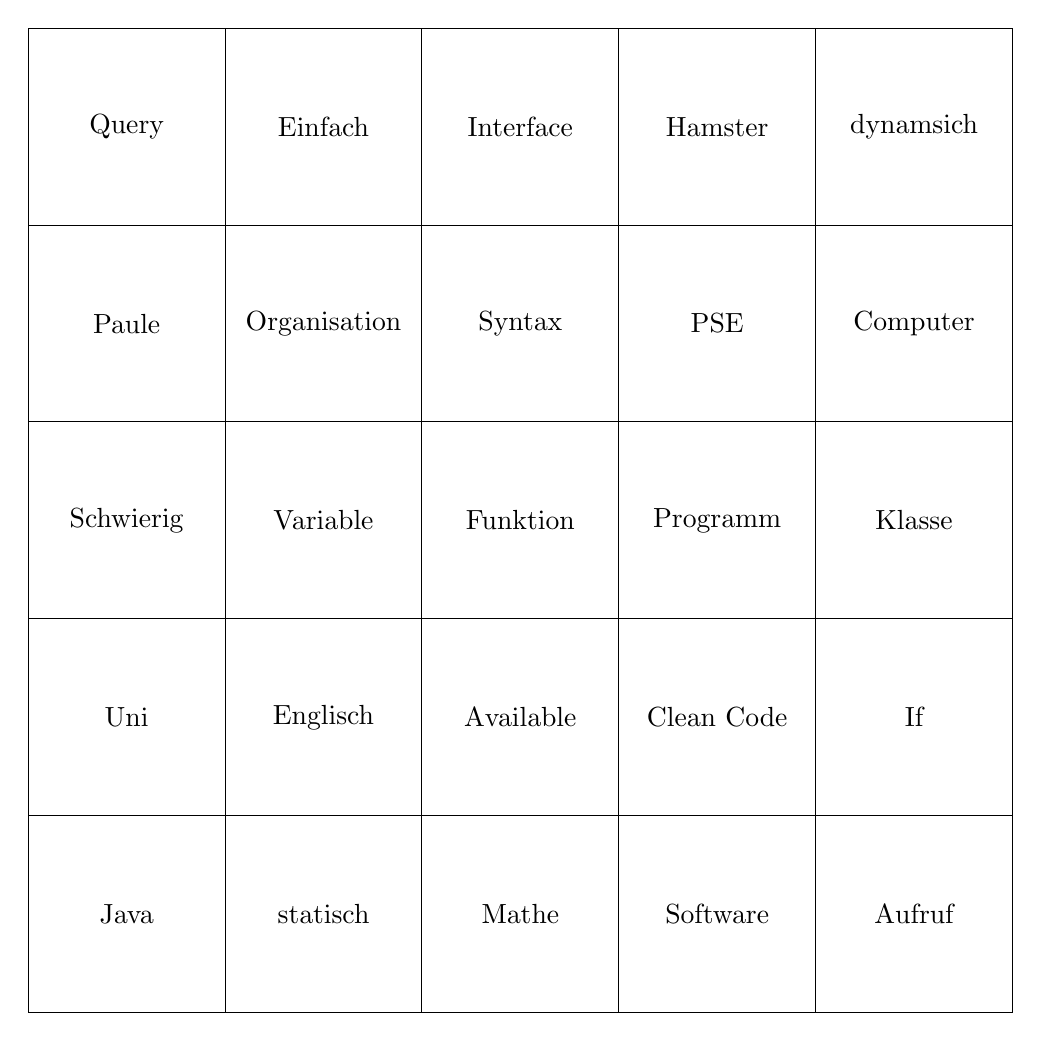
\begin{tikzpicture}[rect/.style={draw, rectangle,anchor=north east, minimum width=\s, minimum height=\s, draw, inner sep=0pt}]
    % First row
    \node[rect] (rect-1-1) at (1*\s,1*\s) {Java};
    \node[rect] (rect-1-2) at (2*\s,1*\s) {statisch};
    \node[rect] (rect-1-3) at (3*\s,1*\s) {Mathe};
    \node[rect] (rect-1-4) at (4*\s,1*\s) {Software};
    \node[rect] (rect-1-5) at (5*\s,1*\s) {Aufruf};

    \node[rect] (rect-1-1) at (1*\s,2*\s) {Uni};
    \node[rect] (rect-1-2) at (2*\s,2*\s) {Englisch};
    \node[rect] (rect-1-3) at (3*\s,2*\s) {Available};
    \node[rect] (rect-1-4) at (4*\s,2*\s) {Clean Code};
    \node[rect] (rect-1-5) at (5*\s,2*\s) {If};

    \node[rect] (rect-1-1) at (1*\s,3*\s) {Schwierig};
    \node[rect] (rect-1-2) at (2*\s,3*\s) {Variable};
    \node[rect] (rect-1-3) at (3*\s,3*\s) {Funktion};
    \node[rect] (rect-1-4) at (4*\s,3*\s) {Programm};
    \node[rect] (rect-1-5) at (5*\s,3*\s) {Klasse};

    \node[rect] (rect-1-1) at (1*\s,4*\s) {Paule};
    \node[rect] (rect-1-2) at (2*\s,4*\s) {Organisation};
    \node[rect] (rect-1-3) at (3*\s,4*\s) {Syntax};
    \node[rect] (rect-1-4) at (4*\s,4*\s) {PSE};
    \node[rect] (rect-1-5) at (5*\s,4*\s) {Computer};

    \node[rect] (rect-1-1) at (1*\s,5*\s) {Query};
    \node[rect] (rect-1-2) at (2*\s,5*\s) {Einfach};
    \node[rect] (rect-1-3) at (3*\s,5*\s) {Interface};
    \node[rect] (rect-1-4) at (4*\s,5*\s) {Hamster};
    \node[rect] (rect-1-5) at (5*\s,5*\s) {dynamsich};

\end{tikzpicture}
\newpage
%
% repeated bingo segment (templated)
\section*{PSE BINGO}
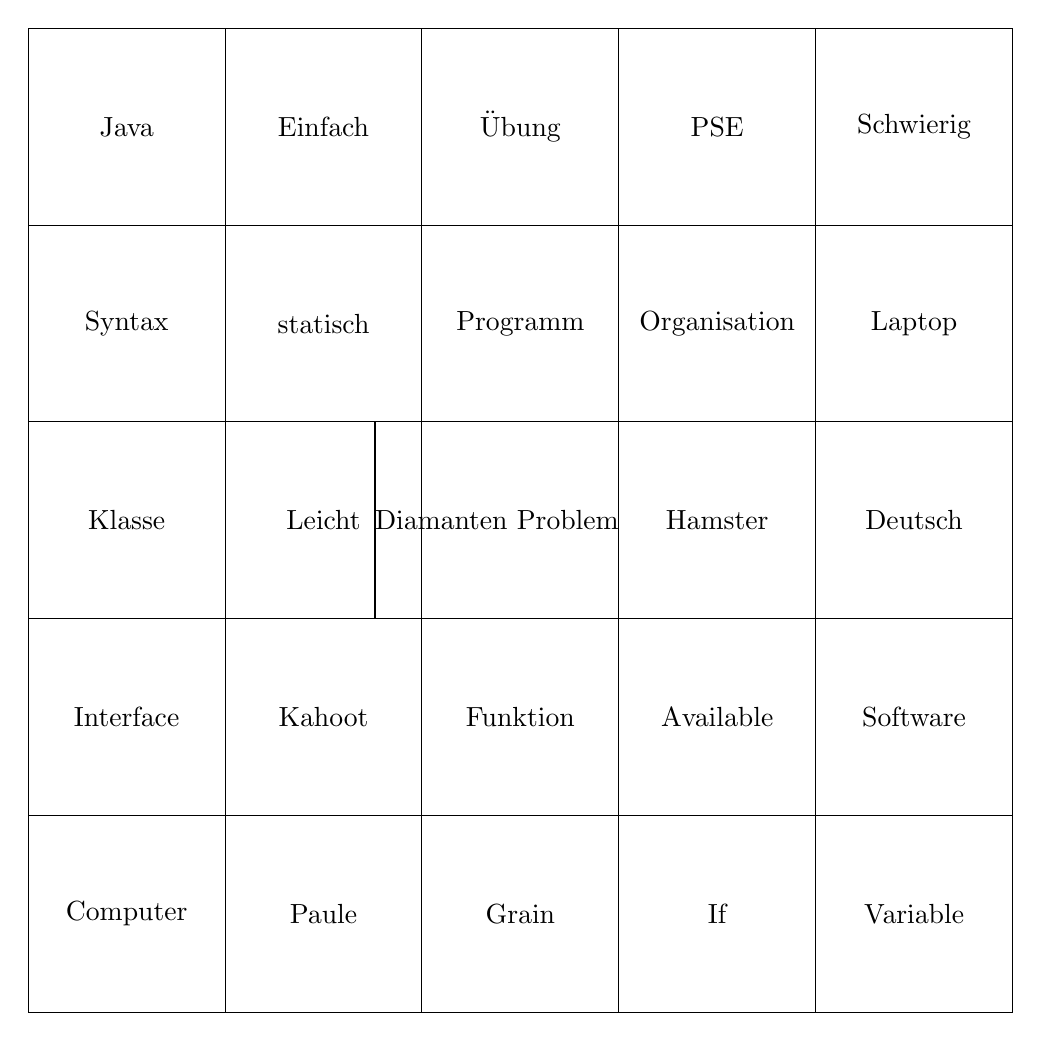
\begin{tikzpicture}[rect/.style={draw, rectangle,anchor=north east, minimum width=\s, minimum height=\s, draw, inner sep=0pt}]
    % First row
    \node[rect] (rect-1-1) at (1*\s,1*\s) {Computer};
    \node[rect] (rect-1-2) at (2*\s,1*\s) {Paule};
    \node[rect] (rect-1-3) at (3*\s,1*\s) {Grain};
    \node[rect] (rect-1-4) at (4*\s,1*\s) {If};
    \node[rect] (rect-1-5) at (5*\s,1*\s) {Variable};

    \node[rect] (rect-1-1) at (1*\s,2*\s) {Interface};
    \node[rect] (rect-1-2) at (2*\s,2*\s) {Kahoot};
    \node[rect] (rect-1-3) at (3*\s,2*\s) {Funktion};
    \node[rect] (rect-1-4) at (4*\s,2*\s) {Available};
    \node[rect] (rect-1-5) at (5*\s,2*\s) {Software};

    \node[rect] (rect-1-1) at (1*\s,3*\s) {Klasse};
    \node[rect] (rect-1-2) at (2*\s,3*\s) {Leicht};
    \node[rect] (rect-1-3) at (3*\s,3*\s) {Diamanten Problem};
    \node[rect] (rect-1-4) at (4*\s,3*\s) {Hamster};
    \node[rect] (rect-1-5) at (5*\s,3*\s) {Deutsch};

    \node[rect] (rect-1-1) at (1*\s,4*\s) {Syntax};
    \node[rect] (rect-1-2) at (2*\s,4*\s) {statisch};
    \node[rect] (rect-1-3) at (3*\s,4*\s) {Programm};
    \node[rect] (rect-1-4) at (4*\s,4*\s) {Organisation};
    \node[rect] (rect-1-5) at (5*\s,4*\s) {Laptop};

    \node[rect] (rect-1-1) at (1*\s,5*\s) {Java};
    \node[rect] (rect-1-2) at (2*\s,5*\s) {Einfach};
    \node[rect] (rect-1-3) at (3*\s,5*\s) {Übung};
    \node[rect] (rect-1-4) at (4*\s,5*\s) {PSE};
    \node[rect] (rect-1-5) at (5*\s,5*\s) {Schwierig};

\end{tikzpicture}
\newpage
%
% repeated bingo segment (templated)
\section*{PSE BINGO}
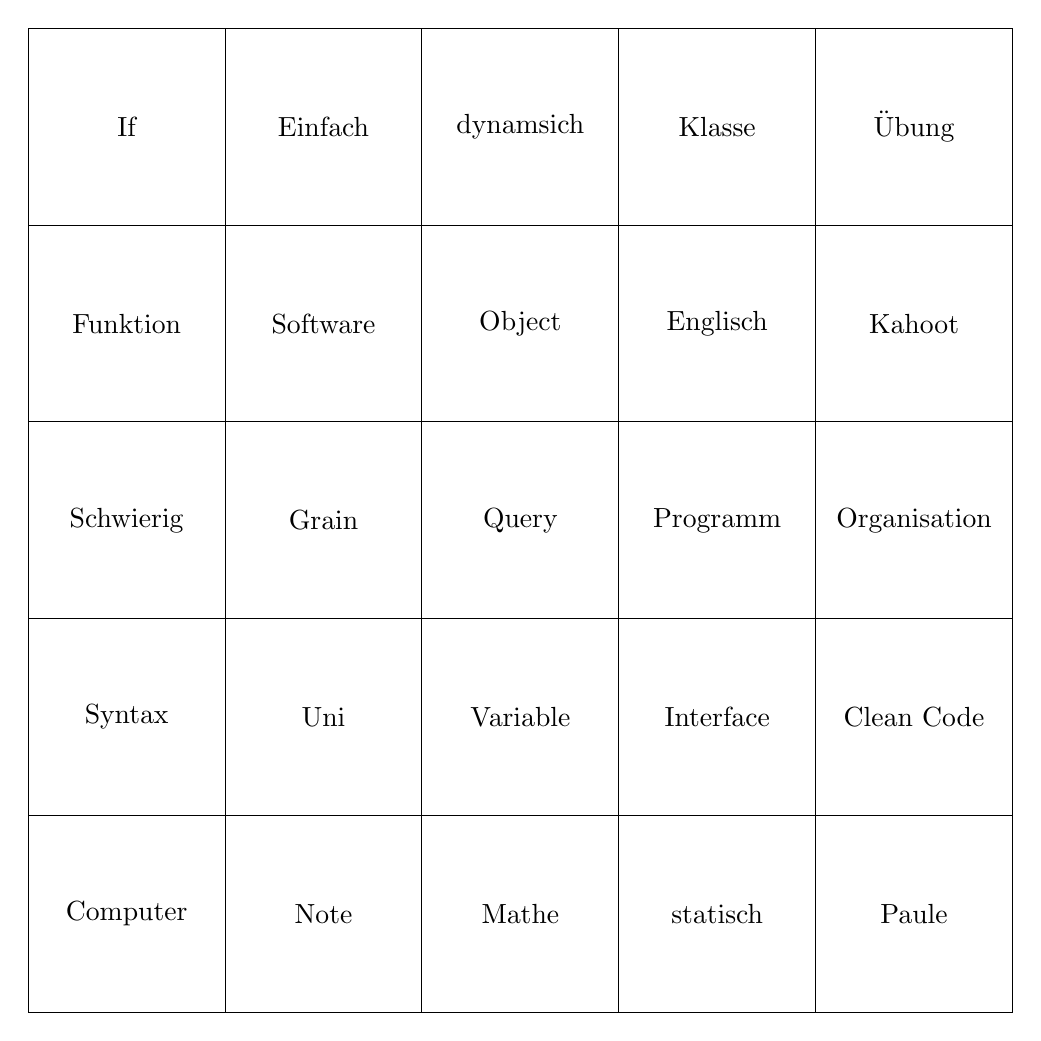
\begin{tikzpicture}[rect/.style={draw, rectangle,anchor=north east, minimum width=\s, minimum height=\s, draw, inner sep=0pt}]
    % First row
    \node[rect] (rect-1-1) at (1*\s,1*\s) {Computer};
    \node[rect] (rect-1-2) at (2*\s,1*\s) {Note};
    \node[rect] (rect-1-3) at (3*\s,1*\s) {Mathe};
    \node[rect] (rect-1-4) at (4*\s,1*\s) {statisch};
    \node[rect] (rect-1-5) at (5*\s,1*\s) {Paule};

    \node[rect] (rect-1-1) at (1*\s,2*\s) {Syntax};
    \node[rect] (rect-1-2) at (2*\s,2*\s) {Uni};
    \node[rect] (rect-1-3) at (3*\s,2*\s) {Variable};
    \node[rect] (rect-1-4) at (4*\s,2*\s) {Interface};
    \node[rect] (rect-1-5) at (5*\s,2*\s) {Clean Code};

    \node[rect] (rect-1-1) at (1*\s,3*\s) {Schwierig};
    \node[rect] (rect-1-2) at (2*\s,3*\s) {Grain};
    \node[rect] (rect-1-3) at (3*\s,3*\s) {Query};
    \node[rect] (rect-1-4) at (4*\s,3*\s) {Programm};
    \node[rect] (rect-1-5) at (5*\s,3*\s) {Organisation};

    \node[rect] (rect-1-1) at (1*\s,4*\s) {Funktion};
    \node[rect] (rect-1-2) at (2*\s,4*\s) {Software};
    \node[rect] (rect-1-3) at (3*\s,4*\s) {Object};
    \node[rect] (rect-1-4) at (4*\s,4*\s) {Englisch};
    \node[rect] (rect-1-5) at (5*\s,4*\s) {Kahoot};

    \node[rect] (rect-1-1) at (1*\s,5*\s) {If};
    \node[rect] (rect-1-2) at (2*\s,5*\s) {Einfach};
    \node[rect] (rect-1-3) at (3*\s,5*\s) {dynamsich};
    \node[rect] (rect-1-4) at (4*\s,5*\s) {Klasse};
    \node[rect] (rect-1-5) at (5*\s,5*\s) {Übung};

\end{tikzpicture}
\newpage
%
% repeated bingo segment (templated)
\section*{PSE BINGO}
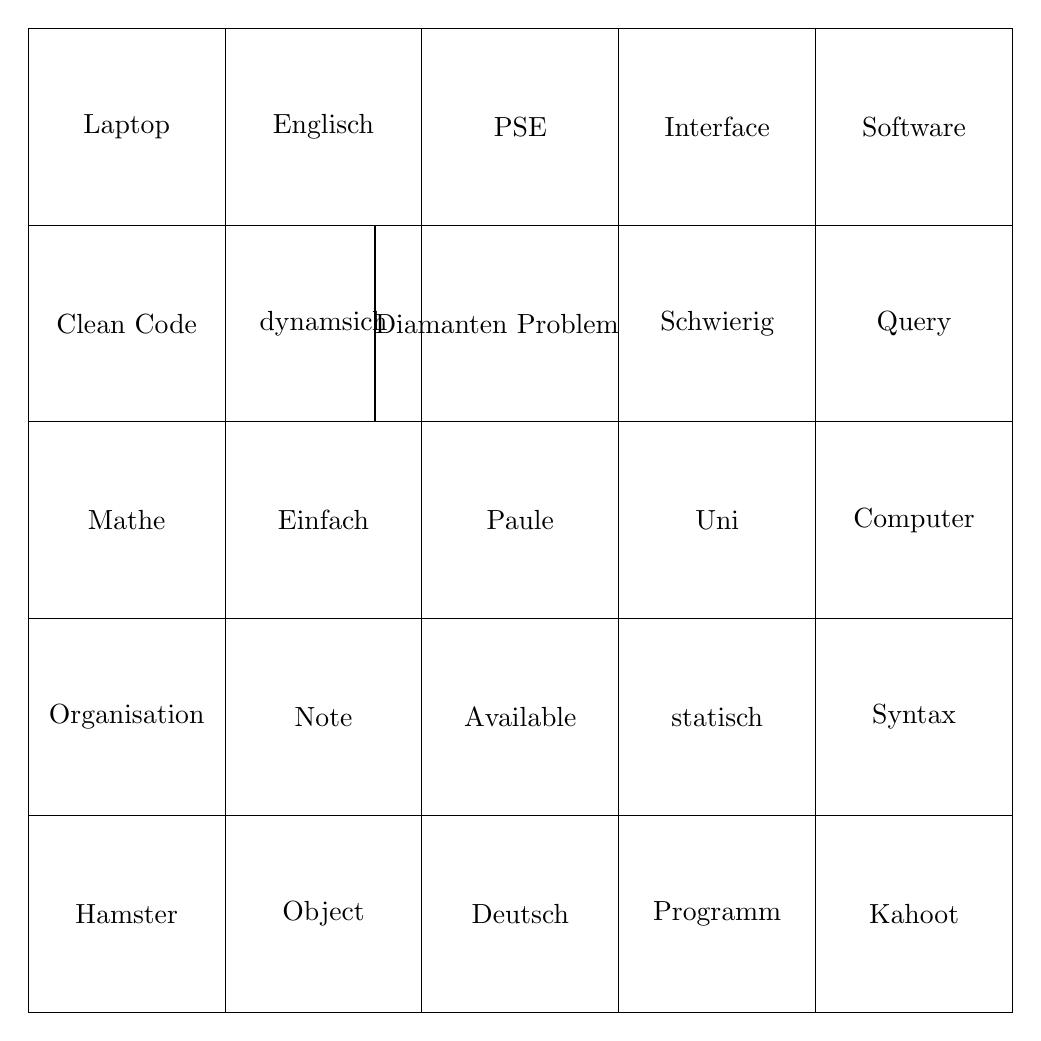
\begin{tikzpicture}[rect/.style={draw, rectangle,anchor=north east, minimum width=\s, minimum height=\s, draw, inner sep=0pt}]
    % First row
    \node[rect] (rect-1-1) at (1*\s,1*\s) {Hamster};
    \node[rect] (rect-1-2) at (2*\s,1*\s) {Object};
    \node[rect] (rect-1-3) at (3*\s,1*\s) {Deutsch};
    \node[rect] (rect-1-4) at (4*\s,1*\s) {Programm};
    \node[rect] (rect-1-5) at (5*\s,1*\s) {Kahoot};

    \node[rect] (rect-1-1) at (1*\s,2*\s) {Organisation};
    \node[rect] (rect-1-2) at (2*\s,2*\s) {Note};
    \node[rect] (rect-1-3) at (3*\s,2*\s) {Available};
    \node[rect] (rect-1-4) at (4*\s,2*\s) {statisch};
    \node[rect] (rect-1-5) at (5*\s,2*\s) {Syntax};

    \node[rect] (rect-1-1) at (1*\s,3*\s) {Mathe};
    \node[rect] (rect-1-2) at (2*\s,3*\s) {Einfach};
    \node[rect] (rect-1-3) at (3*\s,3*\s) {Paule};
    \node[rect] (rect-1-4) at (4*\s,3*\s) {Uni};
    \node[rect] (rect-1-5) at (5*\s,3*\s) {Computer};

    \node[rect] (rect-1-1) at (1*\s,4*\s) {Clean Code};
    \node[rect] (rect-1-2) at (2*\s,4*\s) {dynamsich};
    \node[rect] (rect-1-3) at (3*\s,4*\s) {Diamanten Problem};
    \node[rect] (rect-1-4) at (4*\s,4*\s) {Schwierig};
    \node[rect] (rect-1-5) at (5*\s,4*\s) {Query};

    \node[rect] (rect-1-1) at (1*\s,5*\s) {Laptop};
    \node[rect] (rect-1-2) at (2*\s,5*\s) {Englisch};
    \node[rect] (rect-1-3) at (3*\s,5*\s) {PSE};
    \node[rect] (rect-1-4) at (4*\s,5*\s) {Interface};
    \node[rect] (rect-1-5) at (5*\s,5*\s) {Software};

\end{tikzpicture}
\newpage
%
% repeated bingo segment (templated)
\section*{PSE BINGO}
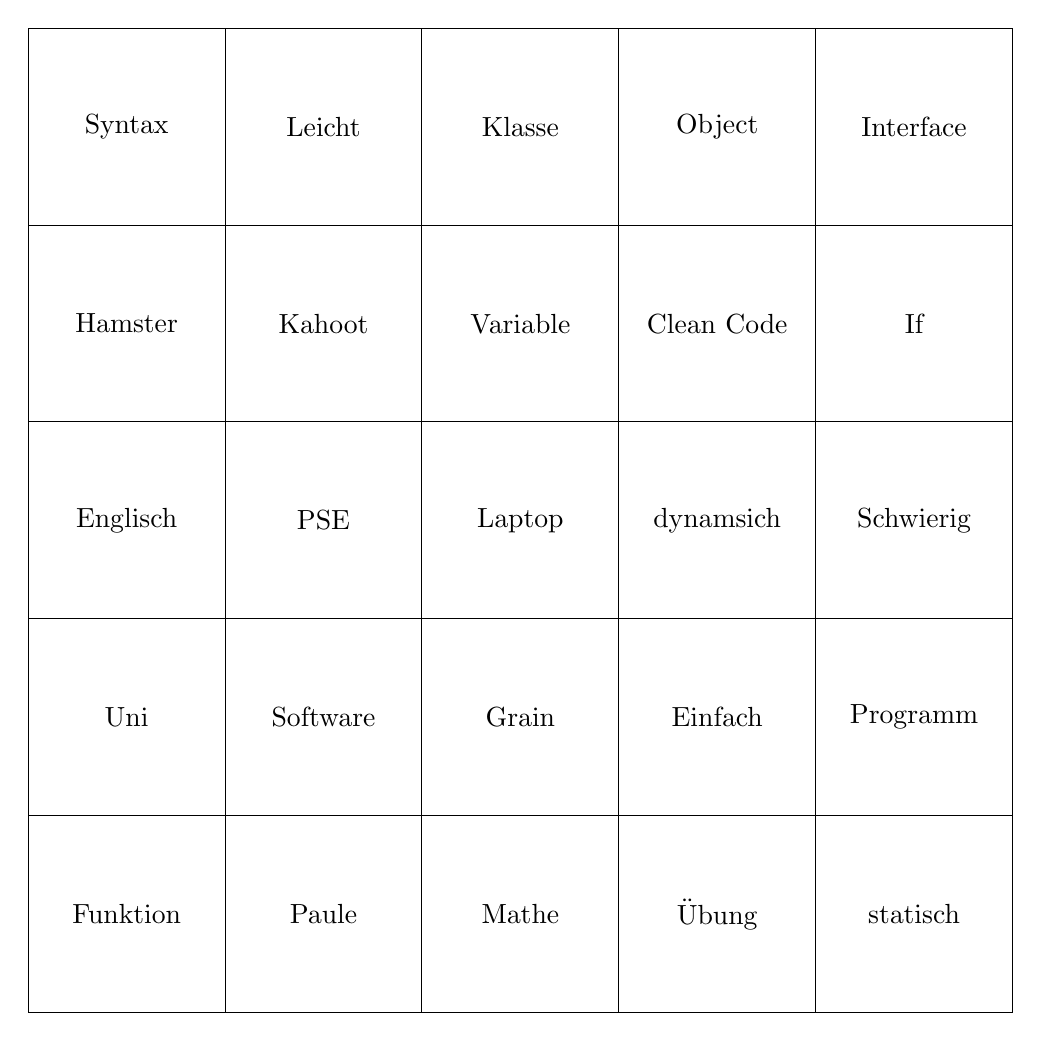
\begin{tikzpicture}[rect/.style={draw, rectangle,anchor=north east, minimum width=\s, minimum height=\s, draw, inner sep=0pt}]
    % First row
    \node[rect] (rect-1-1) at (1*\s,1*\s) {Funktion};
    \node[rect] (rect-1-2) at (2*\s,1*\s) {Paule};
    \node[rect] (rect-1-3) at (3*\s,1*\s) {Mathe};
    \node[rect] (rect-1-4) at (4*\s,1*\s) {Übung};
    \node[rect] (rect-1-5) at (5*\s,1*\s) {statisch};

    \node[rect] (rect-1-1) at (1*\s,2*\s) {Uni};
    \node[rect] (rect-1-2) at (2*\s,2*\s) {Software};
    \node[rect] (rect-1-3) at (3*\s,2*\s) {Grain};
    \node[rect] (rect-1-4) at (4*\s,2*\s) {Einfach};
    \node[rect] (rect-1-5) at (5*\s,2*\s) {Programm};

    \node[rect] (rect-1-1) at (1*\s,3*\s) {Englisch};
    \node[rect] (rect-1-2) at (2*\s,3*\s) {PSE};
    \node[rect] (rect-1-3) at (3*\s,3*\s) {Laptop};
    \node[rect] (rect-1-4) at (4*\s,3*\s) {dynamsich};
    \node[rect] (rect-1-5) at (5*\s,3*\s) {Schwierig};

    \node[rect] (rect-1-1) at (1*\s,4*\s) {Hamster};
    \node[rect] (rect-1-2) at (2*\s,4*\s) {Kahoot};
    \node[rect] (rect-1-3) at (3*\s,4*\s) {Variable};
    \node[rect] (rect-1-4) at (4*\s,4*\s) {Clean Code};
    \node[rect] (rect-1-5) at (5*\s,4*\s) {If};

    \node[rect] (rect-1-1) at (1*\s,5*\s) {Syntax};
    \node[rect] (rect-1-2) at (2*\s,5*\s) {Leicht};
    \node[rect] (rect-1-3) at (3*\s,5*\s) {Klasse};
    \node[rect] (rect-1-4) at (4*\s,5*\s) {Object};
    \node[rect] (rect-1-5) at (5*\s,5*\s) {Interface};

\end{tikzpicture}
\newpage
%
% repeated bingo segment (templated)
\section*{PSE BINGO}
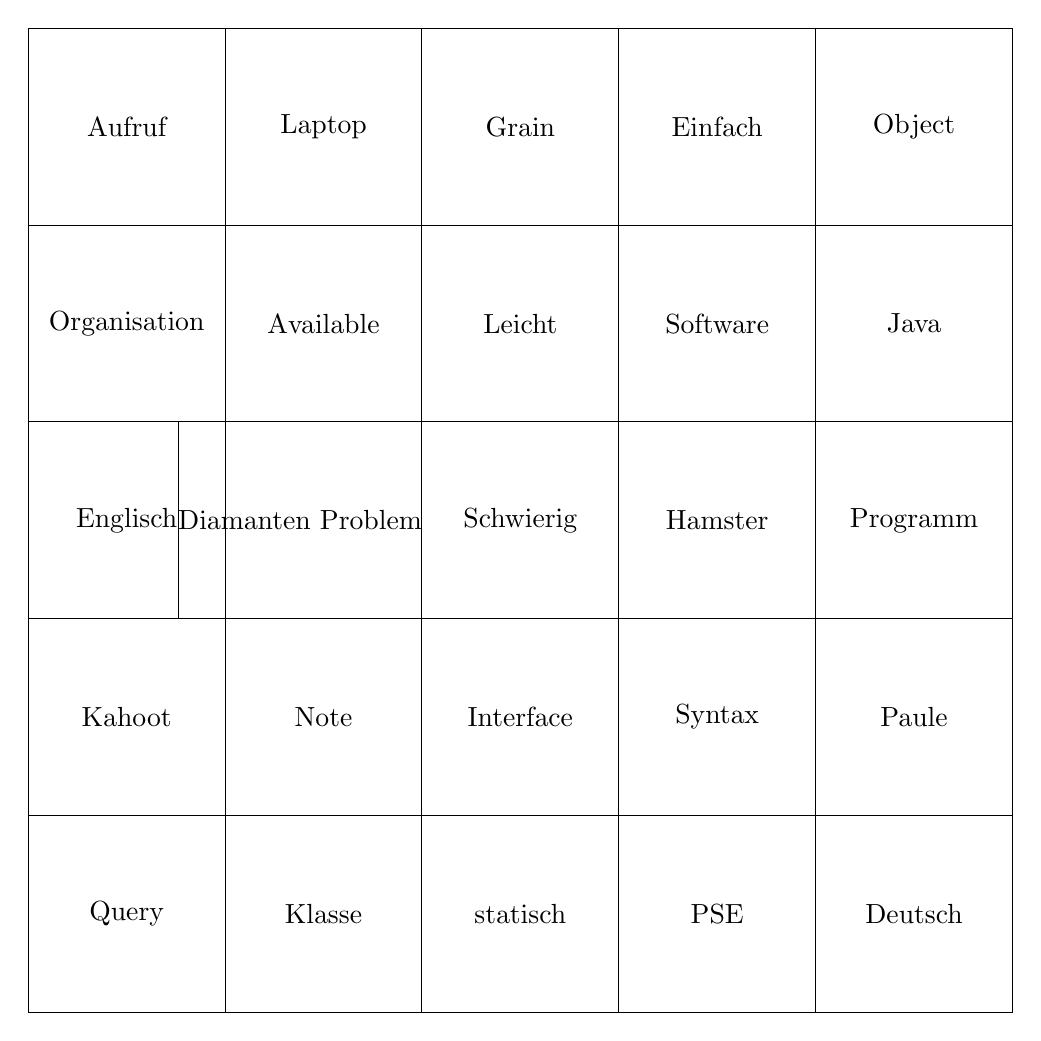
\begin{tikzpicture}[rect/.style={draw, rectangle,anchor=north east, minimum width=\s, minimum height=\s, draw, inner sep=0pt}]
    % First row
    \node[rect] (rect-1-1) at (1*\s,1*\s) {Query};
    \node[rect] (rect-1-2) at (2*\s,1*\s) {Klasse};
    \node[rect] (rect-1-3) at (3*\s,1*\s) {statisch};
    \node[rect] (rect-1-4) at (4*\s,1*\s) {PSE};
    \node[rect] (rect-1-5) at (5*\s,1*\s) {Deutsch};

    \node[rect] (rect-1-1) at (1*\s,2*\s) {Kahoot};
    \node[rect] (rect-1-2) at (2*\s,2*\s) {Note};
    \node[rect] (rect-1-3) at (3*\s,2*\s) {Interface};
    \node[rect] (rect-1-4) at (4*\s,2*\s) {Syntax};
    \node[rect] (rect-1-5) at (5*\s,2*\s) {Paule};

    \node[rect] (rect-1-1) at (1*\s,3*\s) {Englisch};
    \node[rect] (rect-1-2) at (2*\s,3*\s) {Diamanten Problem};
    \node[rect] (rect-1-3) at (3*\s,3*\s) {Schwierig};
    \node[rect] (rect-1-4) at (4*\s,3*\s) {Hamster};
    \node[rect] (rect-1-5) at (5*\s,3*\s) {Programm};

    \node[rect] (rect-1-1) at (1*\s,4*\s) {Organisation};
    \node[rect] (rect-1-2) at (2*\s,4*\s) {Available};
    \node[rect] (rect-1-3) at (3*\s,4*\s) {Leicht};
    \node[rect] (rect-1-4) at (4*\s,4*\s) {Software};
    \node[rect] (rect-1-5) at (5*\s,4*\s) {Java};

    \node[rect] (rect-1-1) at (1*\s,5*\s) {Aufruf};
    \node[rect] (rect-1-2) at (2*\s,5*\s) {Laptop};
    \node[rect] (rect-1-3) at (3*\s,5*\s) {Grain};
    \node[rect] (rect-1-4) at (4*\s,5*\s) {Einfach};
    \node[rect] (rect-1-5) at (5*\s,5*\s) {Object};

\end{tikzpicture}
\newpage
%
% repeated bingo segment (templated)
\section*{PSE BINGO}
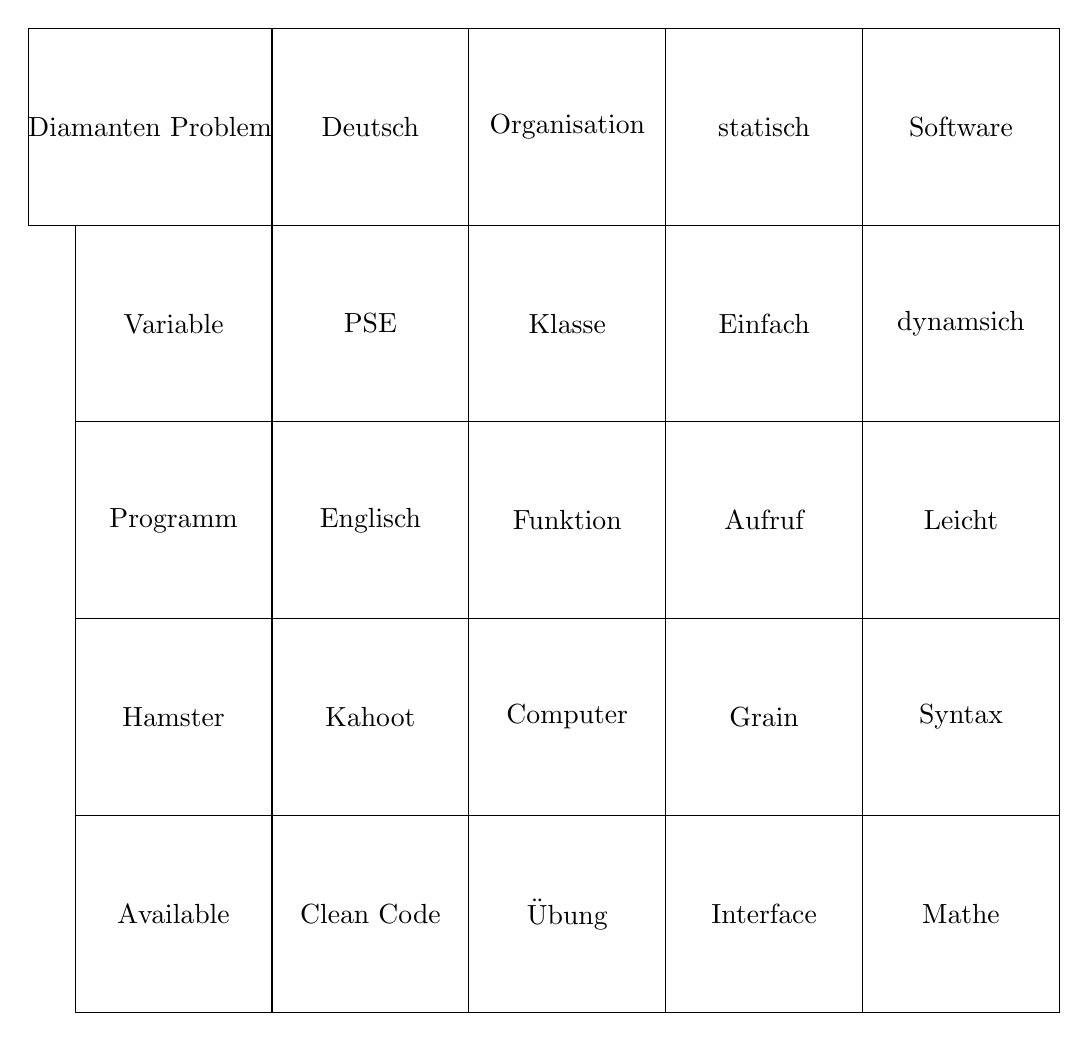
\begin{tikzpicture}[rect/.style={draw, rectangle,anchor=north east, minimum width=\s, minimum height=\s, draw, inner sep=0pt}]
    % First row
    \node[rect] (rect-1-1) at (1*\s,1*\s) {Available};
    \node[rect] (rect-1-2) at (2*\s,1*\s) {Clean Code};
    \node[rect] (rect-1-3) at (3*\s,1*\s) {Übung};
    \node[rect] (rect-1-4) at (4*\s,1*\s) {Interface};
    \node[rect] (rect-1-5) at (5*\s,1*\s) {Mathe};

    \node[rect] (rect-1-1) at (1*\s,2*\s) {Hamster};
    \node[rect] (rect-1-2) at (2*\s,2*\s) {Kahoot};
    \node[rect] (rect-1-3) at (3*\s,2*\s) {Computer};
    \node[rect] (rect-1-4) at (4*\s,2*\s) {Grain};
    \node[rect] (rect-1-5) at (5*\s,2*\s) {Syntax};

    \node[rect] (rect-1-1) at (1*\s,3*\s) {Programm};
    \node[rect] (rect-1-2) at (2*\s,3*\s) {Englisch};
    \node[rect] (rect-1-3) at (3*\s,3*\s) {Funktion};
    \node[rect] (rect-1-4) at (4*\s,3*\s) {Aufruf};
    \node[rect] (rect-1-5) at (5*\s,3*\s) {Leicht};

    \node[rect] (rect-1-1) at (1*\s,4*\s) {Variable};
    \node[rect] (rect-1-2) at (2*\s,4*\s) {PSE};
    \node[rect] (rect-1-3) at (3*\s,4*\s) {Klasse};
    \node[rect] (rect-1-4) at (4*\s,4*\s) {Einfach};
    \node[rect] (rect-1-5) at (5*\s,4*\s) {dynamsich};

    \node[rect] (rect-1-1) at (1*\s,5*\s) {Diamanten Problem};
    \node[rect] (rect-1-2) at (2*\s,5*\s) {Deutsch};
    \node[rect] (rect-1-3) at (3*\s,5*\s) {Organisation};
    \node[rect] (rect-1-4) at (4*\s,5*\s) {statisch};
    \node[rect] (rect-1-5) at (5*\s,5*\s) {Software};

\end{tikzpicture}
\newpage
%
% repeated bingo segment (templated)
\section*{PSE BINGO}
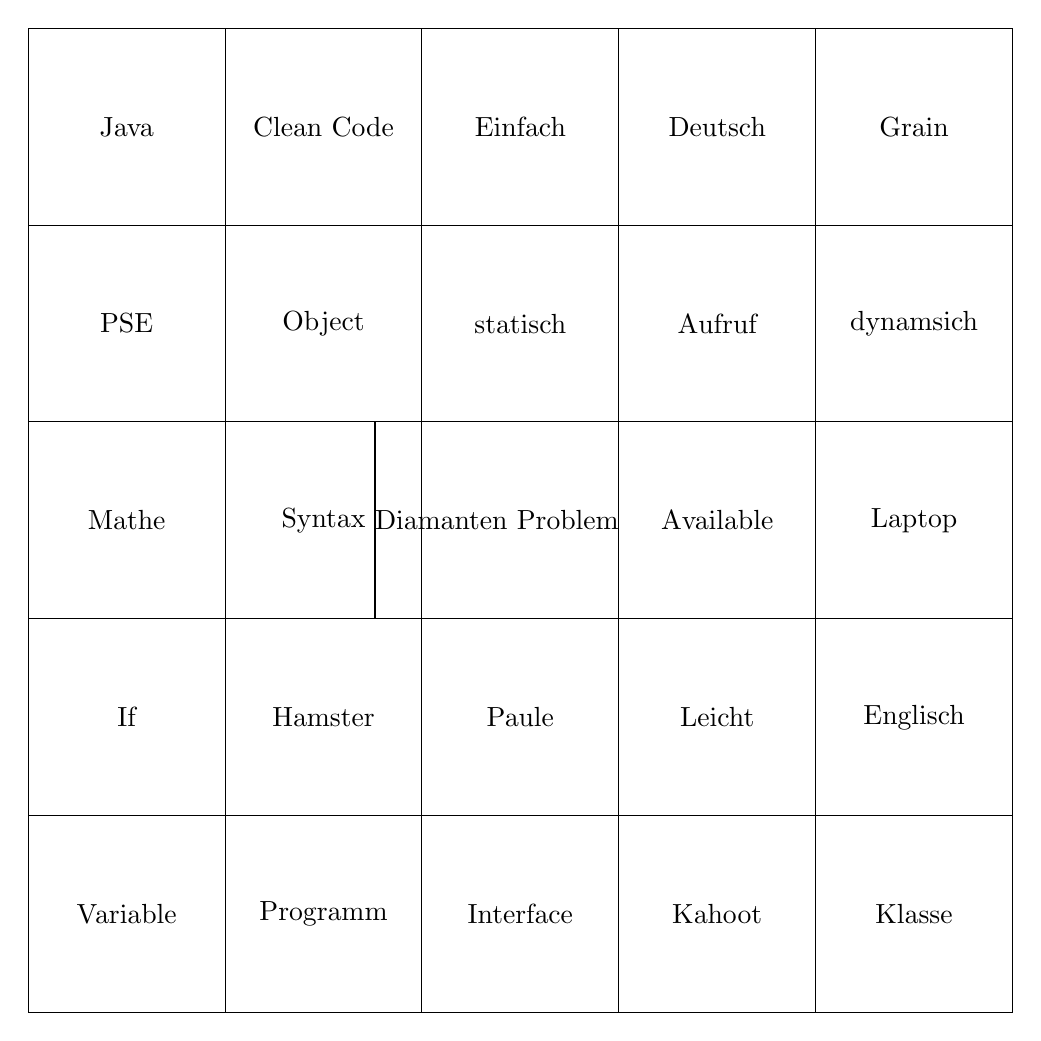
\begin{tikzpicture}[rect/.style={draw, rectangle,anchor=north east, minimum width=\s, minimum height=\s, draw, inner sep=0pt}]
    % First row
    \node[rect] (rect-1-1) at (1*\s,1*\s) {Variable};
    \node[rect] (rect-1-2) at (2*\s,1*\s) {Programm};
    \node[rect] (rect-1-3) at (3*\s,1*\s) {Interface};
    \node[rect] (rect-1-4) at (4*\s,1*\s) {Kahoot};
    \node[rect] (rect-1-5) at (5*\s,1*\s) {Klasse};

    \node[rect] (rect-1-1) at (1*\s,2*\s) {If};
    \node[rect] (rect-1-2) at (2*\s,2*\s) {Hamster};
    \node[rect] (rect-1-3) at (3*\s,2*\s) {Paule};
    \node[rect] (rect-1-4) at (4*\s,2*\s) {Leicht};
    \node[rect] (rect-1-5) at (5*\s,2*\s) {Englisch};

    \node[rect] (rect-1-1) at (1*\s,3*\s) {Mathe};
    \node[rect] (rect-1-2) at (2*\s,3*\s) {Syntax};
    \node[rect] (rect-1-3) at (3*\s,3*\s) {Diamanten Problem};
    \node[rect] (rect-1-4) at (4*\s,3*\s) {Available};
    \node[rect] (rect-1-5) at (5*\s,3*\s) {Laptop};

    \node[rect] (rect-1-1) at (1*\s,4*\s) {PSE};
    \node[rect] (rect-1-2) at (2*\s,4*\s) {Object};
    \node[rect] (rect-1-3) at (3*\s,4*\s) {statisch};
    \node[rect] (rect-1-4) at (4*\s,4*\s) {Aufruf};
    \node[rect] (rect-1-5) at (5*\s,4*\s) {dynamsich};

    \node[rect] (rect-1-1) at (1*\s,5*\s) {Java};
    \node[rect] (rect-1-2) at (2*\s,5*\s) {Clean Code};
    \node[rect] (rect-1-3) at (3*\s,5*\s) {Einfach};
    \node[rect] (rect-1-4) at (4*\s,5*\s) {Deutsch};
    \node[rect] (rect-1-5) at (5*\s,5*\s) {Grain};

\end{tikzpicture}
\newpage
%
% repeated bingo segment (templated)
\section*{PSE BINGO}
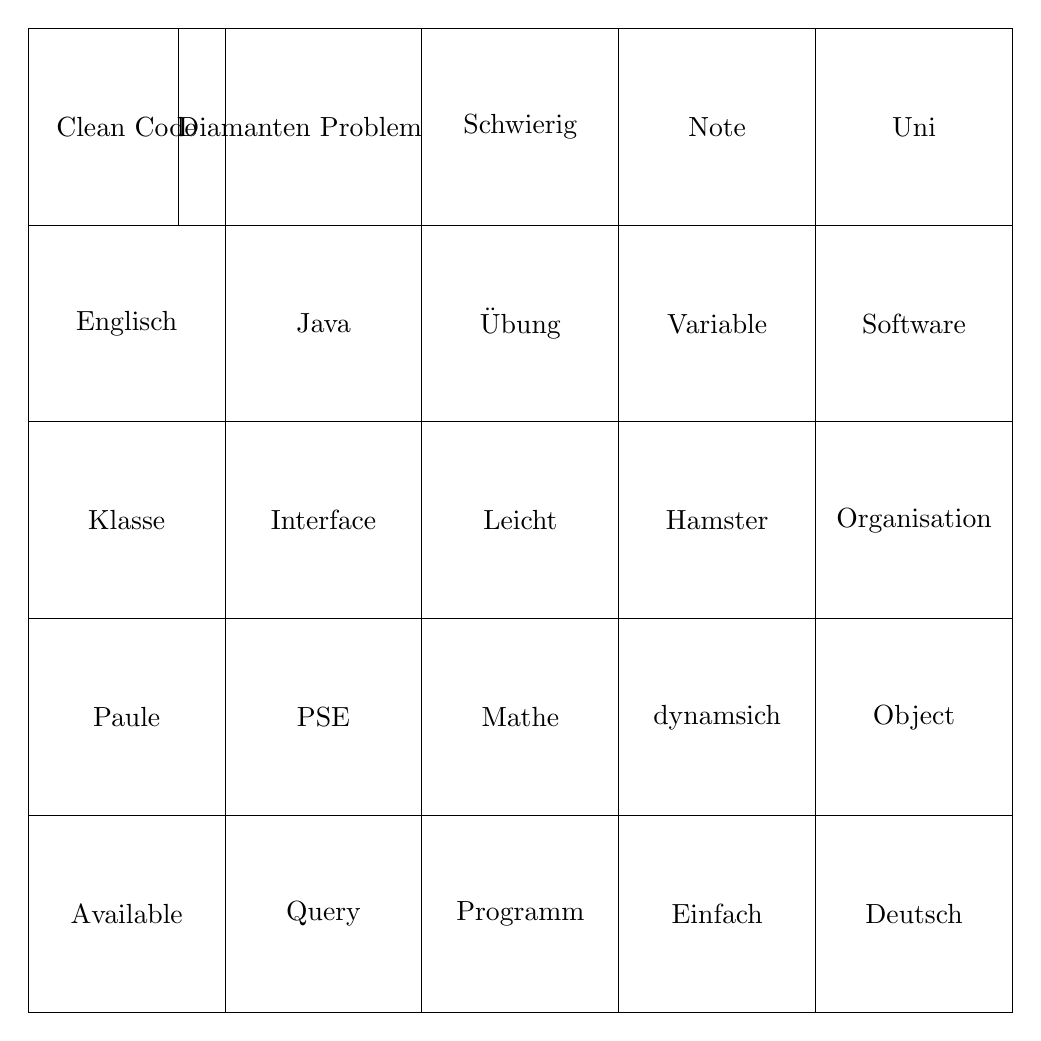
\begin{tikzpicture}[rect/.style={draw, rectangle,anchor=north east, minimum width=\s, minimum height=\s, draw, inner sep=0pt}]
    % First row
    \node[rect] (rect-1-1) at (1*\s,1*\s) {Available};
    \node[rect] (rect-1-2) at (2*\s,1*\s) {Query};
    \node[rect] (rect-1-3) at (3*\s,1*\s) {Programm};
    \node[rect] (rect-1-4) at (4*\s,1*\s) {Einfach};
    \node[rect] (rect-1-5) at (5*\s,1*\s) {Deutsch};

    \node[rect] (rect-1-1) at (1*\s,2*\s) {Paule};
    \node[rect] (rect-1-2) at (2*\s,2*\s) {PSE};
    \node[rect] (rect-1-3) at (3*\s,2*\s) {Mathe};
    \node[rect] (rect-1-4) at (4*\s,2*\s) {dynamsich};
    \node[rect] (rect-1-5) at (5*\s,2*\s) {Object};

    \node[rect] (rect-1-1) at (1*\s,3*\s) {Klasse};
    \node[rect] (rect-1-2) at (2*\s,3*\s) {Interface};
    \node[rect] (rect-1-3) at (3*\s,3*\s) {Leicht};
    \node[rect] (rect-1-4) at (4*\s,3*\s) {Hamster};
    \node[rect] (rect-1-5) at (5*\s,3*\s) {Organisation};

    \node[rect] (rect-1-1) at (1*\s,4*\s) {Englisch};
    \node[rect] (rect-1-2) at (2*\s,4*\s) {Java};
    \node[rect] (rect-1-3) at (3*\s,4*\s) {Übung};
    \node[rect] (rect-1-4) at (4*\s,4*\s) {Variable};
    \node[rect] (rect-1-5) at (5*\s,4*\s) {Software};

    \node[rect] (rect-1-1) at (1*\s,5*\s) {Clean Code};
    \node[rect] (rect-1-2) at (2*\s,5*\s) {Diamanten Problem};
    \node[rect] (rect-1-3) at (3*\s,5*\s) {Schwierig};
    \node[rect] (rect-1-4) at (4*\s,5*\s) {Note};
    \node[rect] (rect-1-5) at (5*\s,5*\s) {Uni};

\end{tikzpicture}
\newpage
%
% repeated bingo segment (templated)
\section*{PSE BINGO}
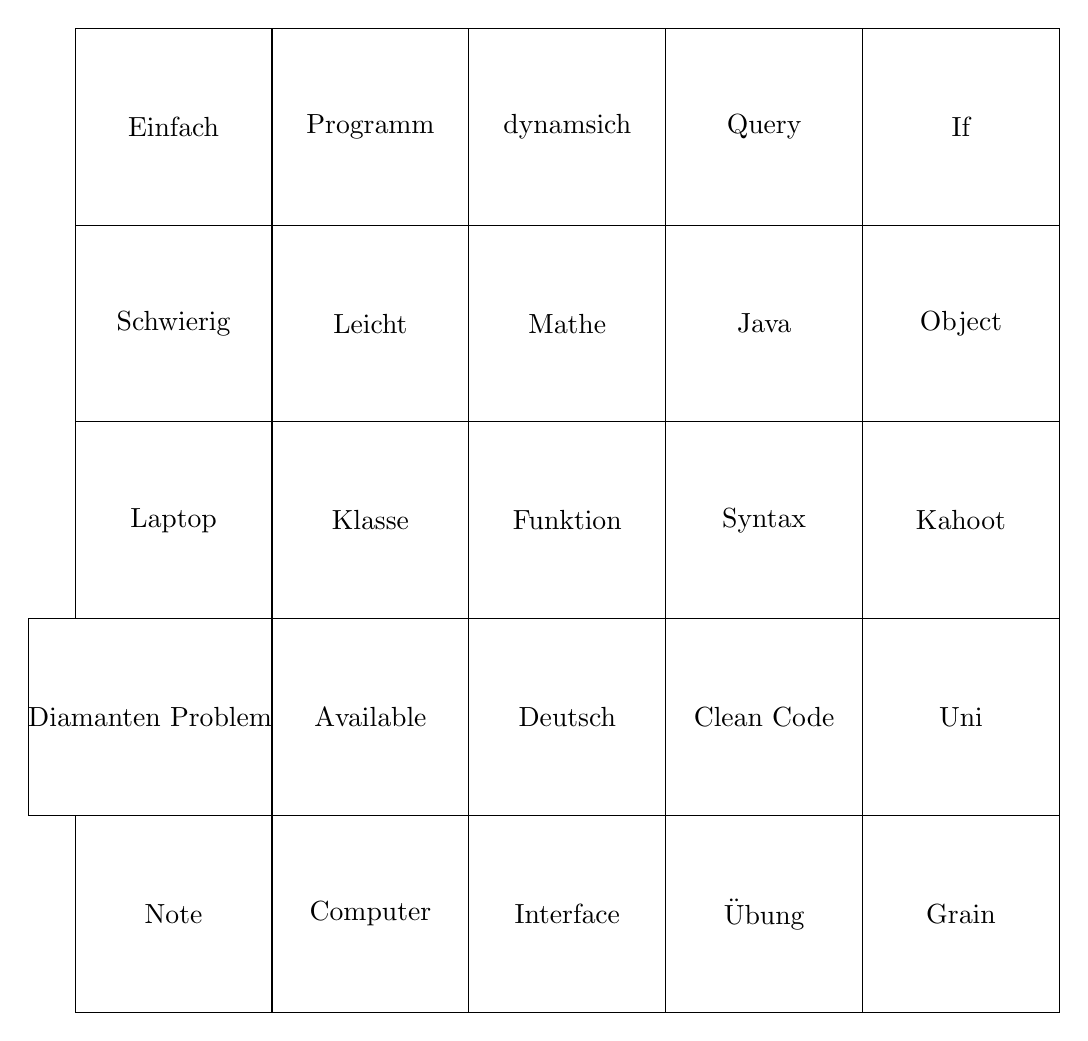
\begin{tikzpicture}[rect/.style={draw, rectangle,anchor=north east, minimum width=\s, minimum height=\s, draw, inner sep=0pt}]
    % First row
    \node[rect] (rect-1-1) at (1*\s,1*\s) {Note};
    \node[rect] (rect-1-2) at (2*\s,1*\s) {Computer};
    \node[rect] (rect-1-3) at (3*\s,1*\s) {Interface};
    \node[rect] (rect-1-4) at (4*\s,1*\s) {Übung};
    \node[rect] (rect-1-5) at (5*\s,1*\s) {Grain};

    \node[rect] (rect-1-1) at (1*\s,2*\s) {Diamanten Problem};
    \node[rect] (rect-1-2) at (2*\s,2*\s) {Available};
    \node[rect] (rect-1-3) at (3*\s,2*\s) {Deutsch};
    \node[rect] (rect-1-4) at (4*\s,2*\s) {Clean Code};
    \node[rect] (rect-1-5) at (5*\s,2*\s) {Uni};

    \node[rect] (rect-1-1) at (1*\s,3*\s) {Laptop};
    \node[rect] (rect-1-2) at (2*\s,3*\s) {Klasse};
    \node[rect] (rect-1-3) at (3*\s,3*\s) {Funktion};
    \node[rect] (rect-1-4) at (4*\s,3*\s) {Syntax};
    \node[rect] (rect-1-5) at (5*\s,3*\s) {Kahoot};

    \node[rect] (rect-1-1) at (1*\s,4*\s) {Schwierig};
    \node[rect] (rect-1-2) at (2*\s,4*\s) {Leicht};
    \node[rect] (rect-1-3) at (3*\s,4*\s) {Mathe};
    \node[rect] (rect-1-4) at (4*\s,4*\s) {Java};
    \node[rect] (rect-1-5) at (5*\s,4*\s) {Object};

    \node[rect] (rect-1-1) at (1*\s,5*\s) {Einfach};
    \node[rect] (rect-1-2) at (2*\s,5*\s) {Programm};
    \node[rect] (rect-1-3) at (3*\s,5*\s) {dynamsich};
    \node[rect] (rect-1-4) at (4*\s,5*\s) {Query};
    \node[rect] (rect-1-5) at (5*\s,5*\s) {If};

\end{tikzpicture}
\newpage
%
% repeated bingo segment (templated)
\section*{PSE BINGO}
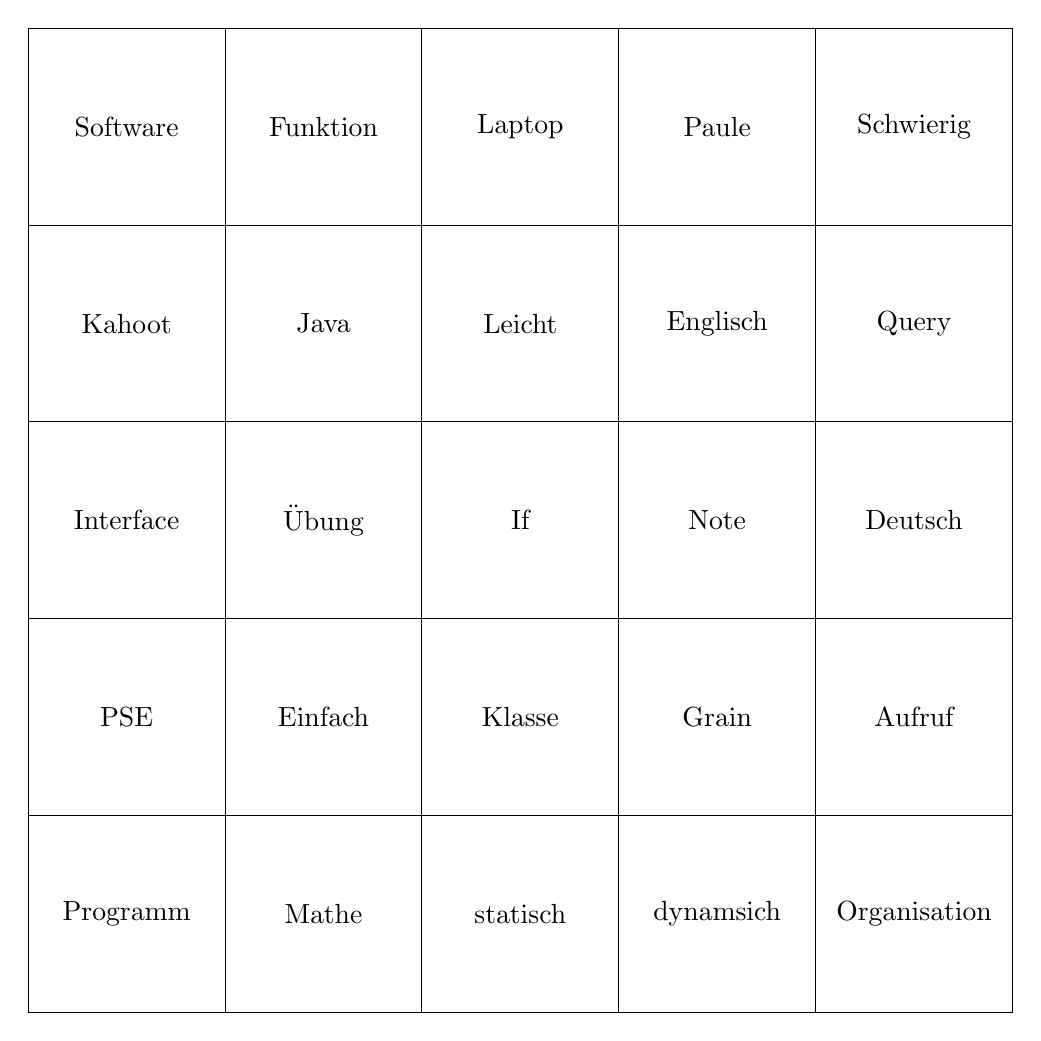
\begin{tikzpicture}[rect/.style={draw, rectangle,anchor=north east, minimum width=\s, minimum height=\s, draw, inner sep=0pt}]
    % First row
    \node[rect] (rect-1-1) at (1*\s,1*\s) {Programm};
    \node[rect] (rect-1-2) at (2*\s,1*\s) {Mathe};
    \node[rect] (rect-1-3) at (3*\s,1*\s) {statisch};
    \node[rect] (rect-1-4) at (4*\s,1*\s) {dynamsich};
    \node[rect] (rect-1-5) at (5*\s,1*\s) {Organisation};

    \node[rect] (rect-1-1) at (1*\s,2*\s) {PSE};
    \node[rect] (rect-1-2) at (2*\s,2*\s) {Einfach};
    \node[rect] (rect-1-3) at (3*\s,2*\s) {Klasse};
    \node[rect] (rect-1-4) at (4*\s,2*\s) {Grain};
    \node[rect] (rect-1-5) at (5*\s,2*\s) {Aufruf};

    \node[rect] (rect-1-1) at (1*\s,3*\s) {Interface};
    \node[rect] (rect-1-2) at (2*\s,3*\s) {Übung};
    \node[rect] (rect-1-3) at (3*\s,3*\s) {If};
    \node[rect] (rect-1-4) at (4*\s,3*\s) {Note};
    \node[rect] (rect-1-5) at (5*\s,3*\s) {Deutsch};

    \node[rect] (rect-1-1) at (1*\s,4*\s) {Kahoot};
    \node[rect] (rect-1-2) at (2*\s,4*\s) {Java};
    \node[rect] (rect-1-3) at (3*\s,4*\s) {Leicht};
    \node[rect] (rect-1-4) at (4*\s,4*\s) {Englisch};
    \node[rect] (rect-1-5) at (5*\s,4*\s) {Query};

    \node[rect] (rect-1-1) at (1*\s,5*\s) {Software};
    \node[rect] (rect-1-2) at (2*\s,5*\s) {Funktion};
    \node[rect] (rect-1-3) at (3*\s,5*\s) {Laptop};
    \node[rect] (rect-1-4) at (4*\s,5*\s) {Paule};
    \node[rect] (rect-1-5) at (5*\s,5*\s) {Schwierig};

\end{tikzpicture}
\newpage
%
% repeated bingo segment (templated)
\section*{PSE BINGO}
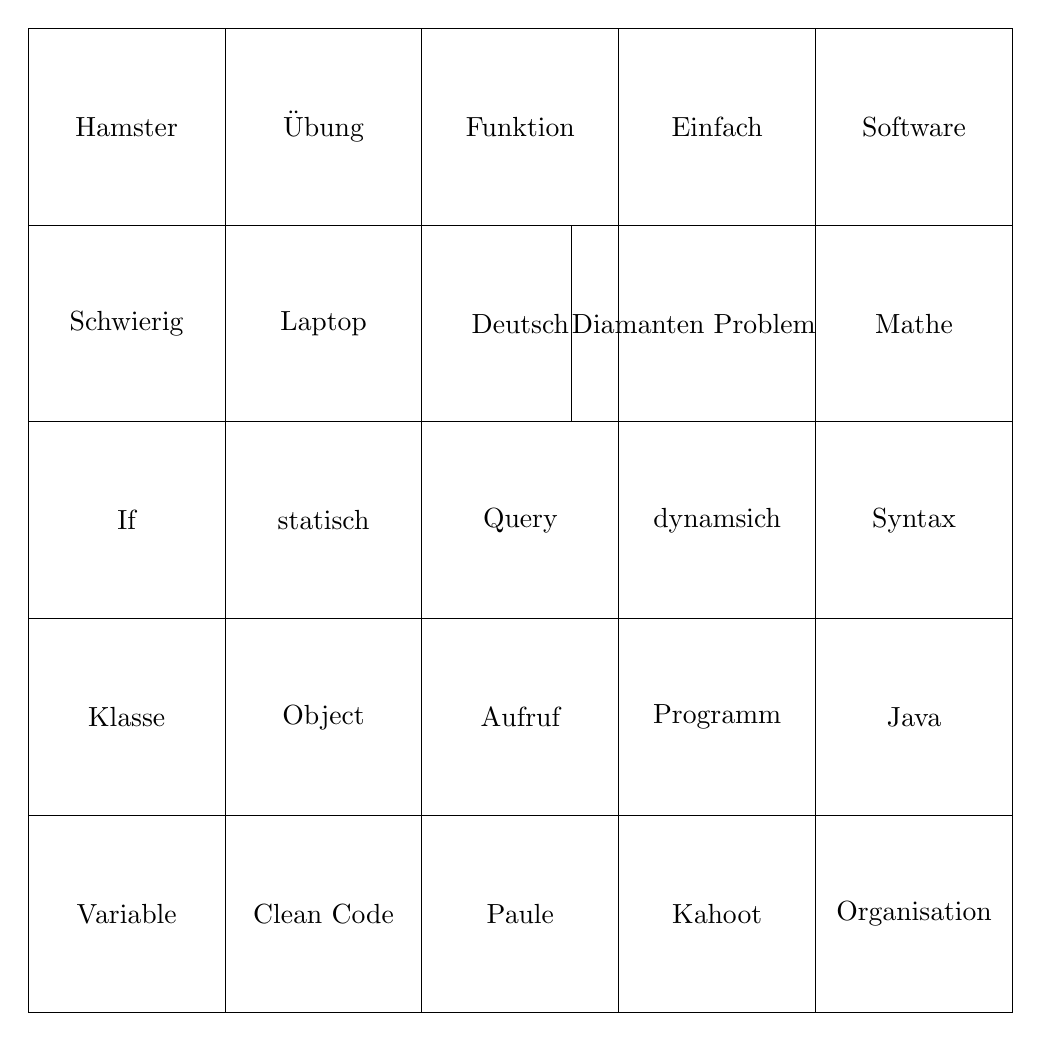
\begin{tikzpicture}[rect/.style={draw, rectangle,anchor=north east, minimum width=\s, minimum height=\s, draw, inner sep=0pt}]
    % First row
    \node[rect] (rect-1-1) at (1*\s,1*\s) {Variable};
    \node[rect] (rect-1-2) at (2*\s,1*\s) {Clean Code};
    \node[rect] (rect-1-3) at (3*\s,1*\s) {Paule};
    \node[rect] (rect-1-4) at (4*\s,1*\s) {Kahoot};
    \node[rect] (rect-1-5) at (5*\s,1*\s) {Organisation};

    \node[rect] (rect-1-1) at (1*\s,2*\s) {Klasse};
    \node[rect] (rect-1-2) at (2*\s,2*\s) {Object};
    \node[rect] (rect-1-3) at (3*\s,2*\s) {Aufruf};
    \node[rect] (rect-1-4) at (4*\s,2*\s) {Programm};
    \node[rect] (rect-1-5) at (5*\s,2*\s) {Java};

    \node[rect] (rect-1-1) at (1*\s,3*\s) {If};
    \node[rect] (rect-1-2) at (2*\s,3*\s) {statisch};
    \node[rect] (rect-1-3) at (3*\s,3*\s) {Query};
    \node[rect] (rect-1-4) at (4*\s,3*\s) {dynamsich};
    \node[rect] (rect-1-5) at (5*\s,3*\s) {Syntax};

    \node[rect] (rect-1-1) at (1*\s,4*\s) {Schwierig};
    \node[rect] (rect-1-2) at (2*\s,4*\s) {Laptop};
    \node[rect] (rect-1-3) at (3*\s,4*\s) {Deutsch};
    \node[rect] (rect-1-4) at (4*\s,4*\s) {Diamanten Problem};
    \node[rect] (rect-1-5) at (5*\s,4*\s) {Mathe};

    \node[rect] (rect-1-1) at (1*\s,5*\s) {Hamster};
    \node[rect] (rect-1-2) at (2*\s,5*\s) {Übung};
    \node[rect] (rect-1-3) at (3*\s,5*\s) {Funktion};
    \node[rect] (rect-1-4) at (4*\s,5*\s) {Einfach};
    \node[rect] (rect-1-5) at (5*\s,5*\s) {Software};

\end{tikzpicture}
\newpage
%
% repeated bingo segment (templated)
\section*{PSE BINGO}
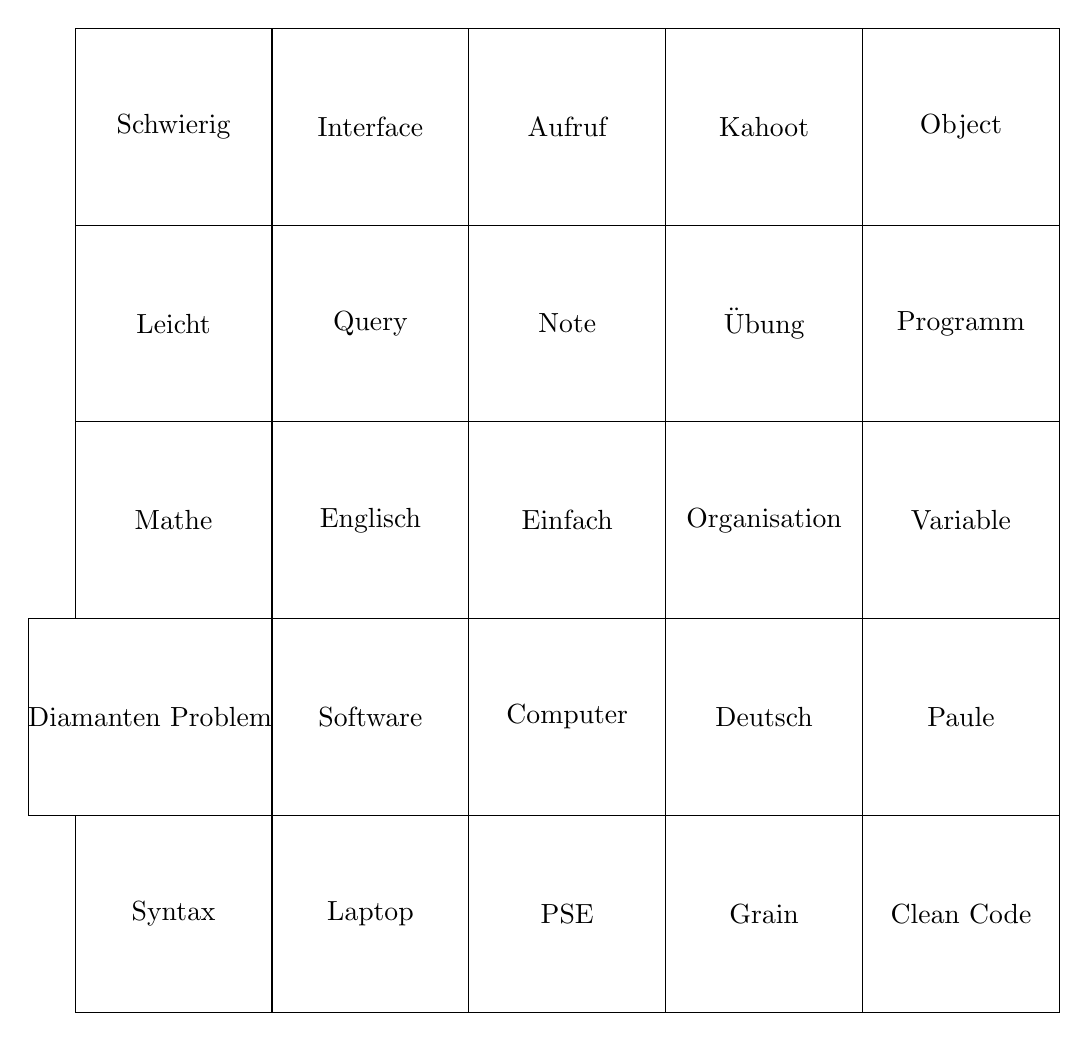
\begin{tikzpicture}[rect/.style={draw, rectangle,anchor=north east, minimum width=\s, minimum height=\s, draw, inner sep=0pt}]
    % First row
    \node[rect] (rect-1-1) at (1*\s,1*\s) {Syntax};
    \node[rect] (rect-1-2) at (2*\s,1*\s) {Laptop};
    \node[rect] (rect-1-3) at (3*\s,1*\s) {PSE};
    \node[rect] (rect-1-4) at (4*\s,1*\s) {Grain};
    \node[rect] (rect-1-5) at (5*\s,1*\s) {Clean Code};

    \node[rect] (rect-1-1) at (1*\s,2*\s) {Diamanten Problem};
    \node[rect] (rect-1-2) at (2*\s,2*\s) {Software};
    \node[rect] (rect-1-3) at (3*\s,2*\s) {Computer};
    \node[rect] (rect-1-4) at (4*\s,2*\s) {Deutsch};
    \node[rect] (rect-1-5) at (5*\s,2*\s) {Paule};

    \node[rect] (rect-1-1) at (1*\s,3*\s) {Mathe};
    \node[rect] (rect-1-2) at (2*\s,3*\s) {Englisch};
    \node[rect] (rect-1-3) at (3*\s,3*\s) {Einfach};
    \node[rect] (rect-1-4) at (4*\s,3*\s) {Organisation};
    \node[rect] (rect-1-5) at (5*\s,3*\s) {Variable};

    \node[rect] (rect-1-1) at (1*\s,4*\s) {Leicht};
    \node[rect] (rect-1-2) at (2*\s,4*\s) {Query};
    \node[rect] (rect-1-3) at (3*\s,4*\s) {Note};
    \node[rect] (rect-1-4) at (4*\s,4*\s) {Übung};
    \node[rect] (rect-1-5) at (5*\s,4*\s) {Programm};

    \node[rect] (rect-1-1) at (1*\s,5*\s) {Schwierig};
    \node[rect] (rect-1-2) at (2*\s,5*\s) {Interface};
    \node[rect] (rect-1-3) at (3*\s,5*\s) {Aufruf};
    \node[rect] (rect-1-4) at (4*\s,5*\s) {Kahoot};
    \node[rect] (rect-1-5) at (5*\s,5*\s) {Object};

\end{tikzpicture}
\newpage
%
% repeated bingo segment (templated)
\section*{PSE BINGO}
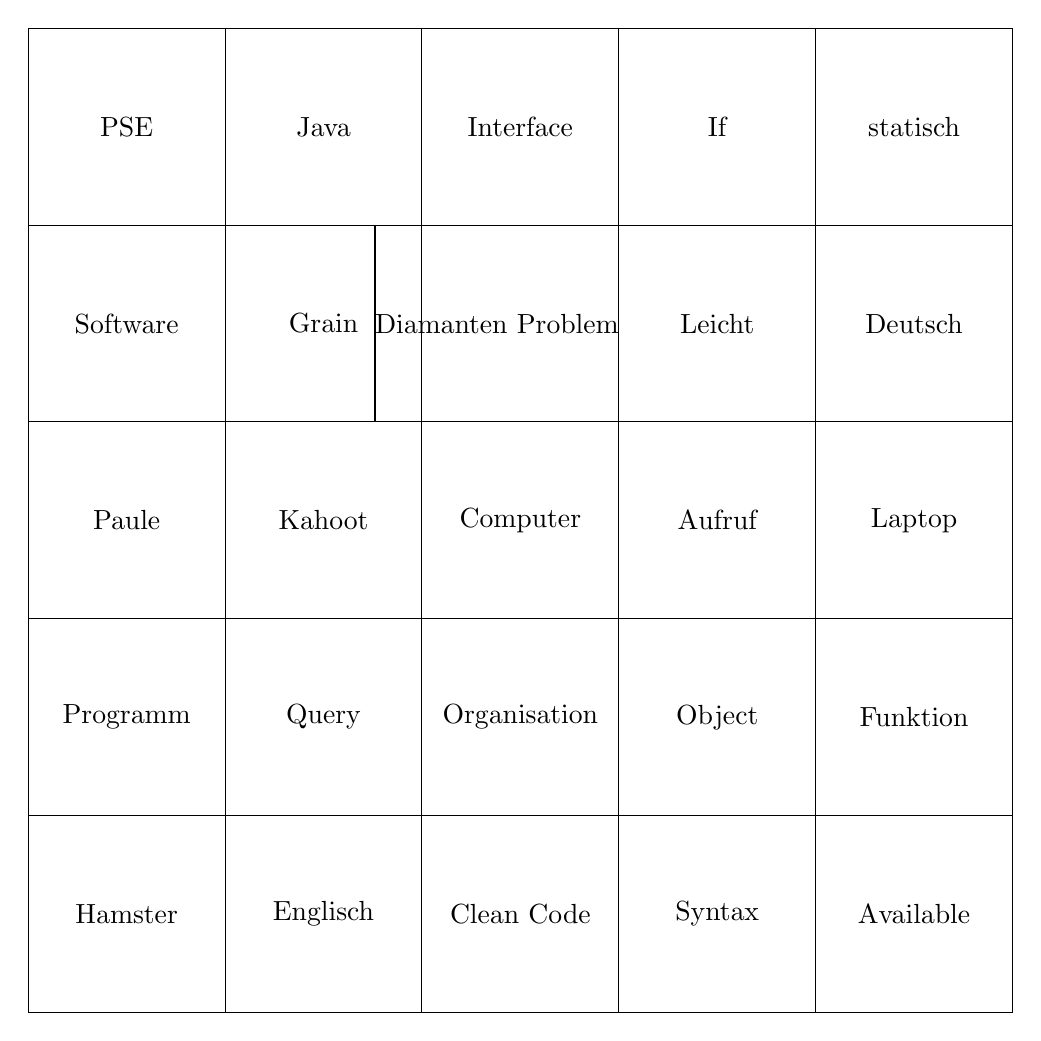
\begin{tikzpicture}[rect/.style={draw, rectangle,anchor=north east, minimum width=\s, minimum height=\s, draw, inner sep=0pt}]
    % First row
    \node[rect] (rect-1-1) at (1*\s,1*\s) {Hamster};
    \node[rect] (rect-1-2) at (2*\s,1*\s) {Englisch};
    \node[rect] (rect-1-3) at (3*\s,1*\s) {Clean Code};
    \node[rect] (rect-1-4) at (4*\s,1*\s) {Syntax};
    \node[rect] (rect-1-5) at (5*\s,1*\s) {Available};

    \node[rect] (rect-1-1) at (1*\s,2*\s) {Programm};
    \node[rect] (rect-1-2) at (2*\s,2*\s) {Query};
    \node[rect] (rect-1-3) at (3*\s,2*\s) {Organisation};
    \node[rect] (rect-1-4) at (4*\s,2*\s) {Object};
    \node[rect] (rect-1-5) at (5*\s,2*\s) {Funktion};

    \node[rect] (rect-1-1) at (1*\s,3*\s) {Paule};
    \node[rect] (rect-1-2) at (2*\s,3*\s) {Kahoot};
    \node[rect] (rect-1-3) at (3*\s,3*\s) {Computer};
    \node[rect] (rect-1-4) at (4*\s,3*\s) {Aufruf};
    \node[rect] (rect-1-5) at (5*\s,3*\s) {Laptop};

    \node[rect] (rect-1-1) at (1*\s,4*\s) {Software};
    \node[rect] (rect-1-2) at (2*\s,4*\s) {Grain};
    \node[rect] (rect-1-3) at (3*\s,4*\s) {Diamanten Problem};
    \node[rect] (rect-1-4) at (4*\s,4*\s) {Leicht};
    \node[rect] (rect-1-5) at (5*\s,4*\s) {Deutsch};

    \node[rect] (rect-1-1) at (1*\s,5*\s) {PSE};
    \node[rect] (rect-1-2) at (2*\s,5*\s) {Java};
    \node[rect] (rect-1-3) at (3*\s,5*\s) {Interface};
    \node[rect] (rect-1-4) at (4*\s,5*\s) {If};
    \node[rect] (rect-1-5) at (5*\s,5*\s) {statisch};

\end{tikzpicture}
\newpage
%
% repeated bingo segment (templated)
\section*{PSE BINGO}
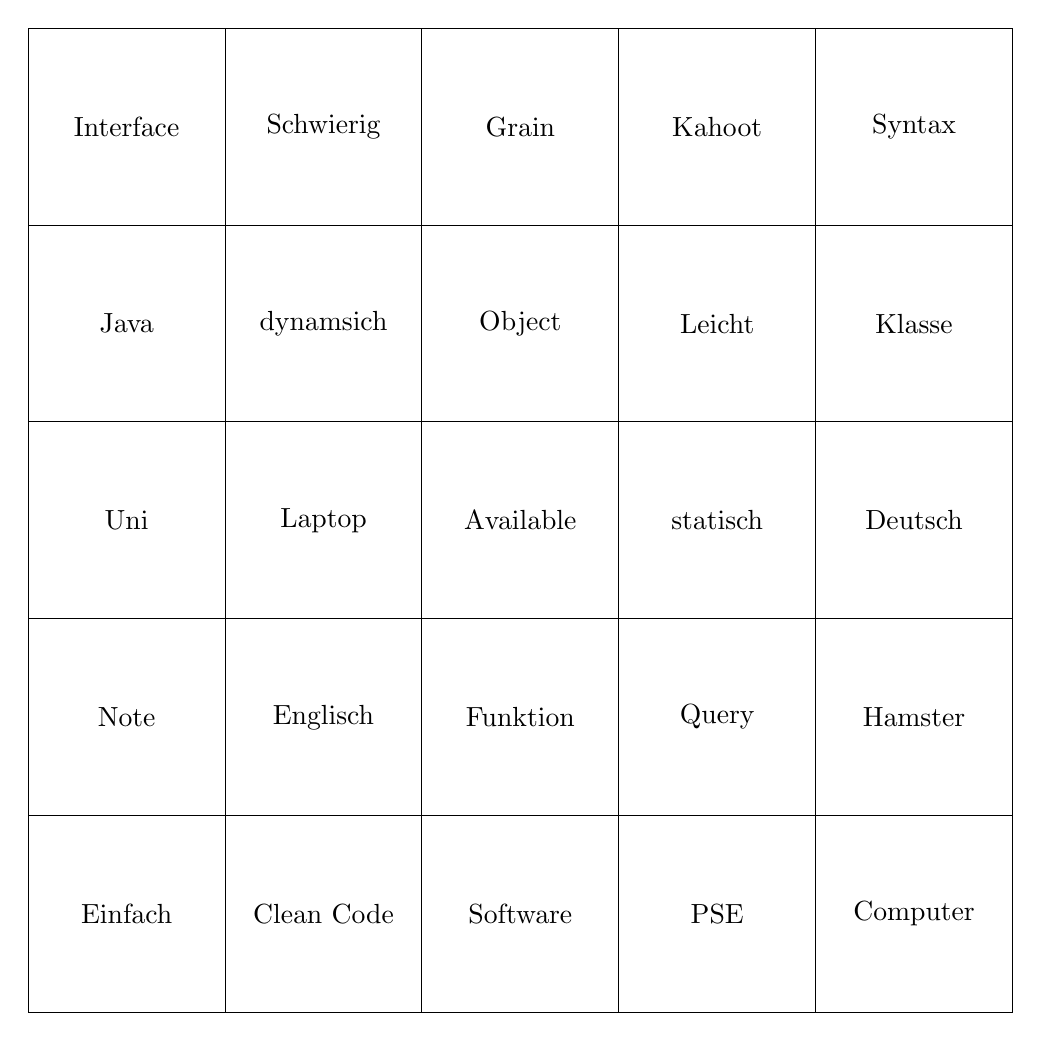
\begin{tikzpicture}[rect/.style={draw, rectangle,anchor=north east, minimum width=\s, minimum height=\s, draw, inner sep=0pt}]
    % First row
    \node[rect] (rect-1-1) at (1*\s,1*\s) {Einfach};
    \node[rect] (rect-1-2) at (2*\s,1*\s) {Clean Code};
    \node[rect] (rect-1-3) at (3*\s,1*\s) {Software};
    \node[rect] (rect-1-4) at (4*\s,1*\s) {PSE};
    \node[rect] (rect-1-5) at (5*\s,1*\s) {Computer};

    \node[rect] (rect-1-1) at (1*\s,2*\s) {Note};
    \node[rect] (rect-1-2) at (2*\s,2*\s) {Englisch};
    \node[rect] (rect-1-3) at (3*\s,2*\s) {Funktion};
    \node[rect] (rect-1-4) at (4*\s,2*\s) {Query};
    \node[rect] (rect-1-5) at (5*\s,2*\s) {Hamster};

    \node[rect] (rect-1-1) at (1*\s,3*\s) {Uni};
    \node[rect] (rect-1-2) at (2*\s,3*\s) {Laptop};
    \node[rect] (rect-1-3) at (3*\s,3*\s) {Available};
    \node[rect] (rect-1-4) at (4*\s,3*\s) {statisch};
    \node[rect] (rect-1-5) at (5*\s,3*\s) {Deutsch};

    \node[rect] (rect-1-1) at (1*\s,4*\s) {Java};
    \node[rect] (rect-1-2) at (2*\s,4*\s) {dynamsich};
    \node[rect] (rect-1-3) at (3*\s,4*\s) {Object};
    \node[rect] (rect-1-4) at (4*\s,4*\s) {Leicht};
    \node[rect] (rect-1-5) at (5*\s,4*\s) {Klasse};

    \node[rect] (rect-1-1) at (1*\s,5*\s) {Interface};
    \node[rect] (rect-1-2) at (2*\s,5*\s) {Schwierig};
    \node[rect] (rect-1-3) at (3*\s,5*\s) {Grain};
    \node[rect] (rect-1-4) at (4*\s,5*\s) {Kahoot};
    \node[rect] (rect-1-5) at (5*\s,5*\s) {Syntax};

\end{tikzpicture}
\newpage
%
% repeated bingo segment (templated)
\section*{PSE BINGO}
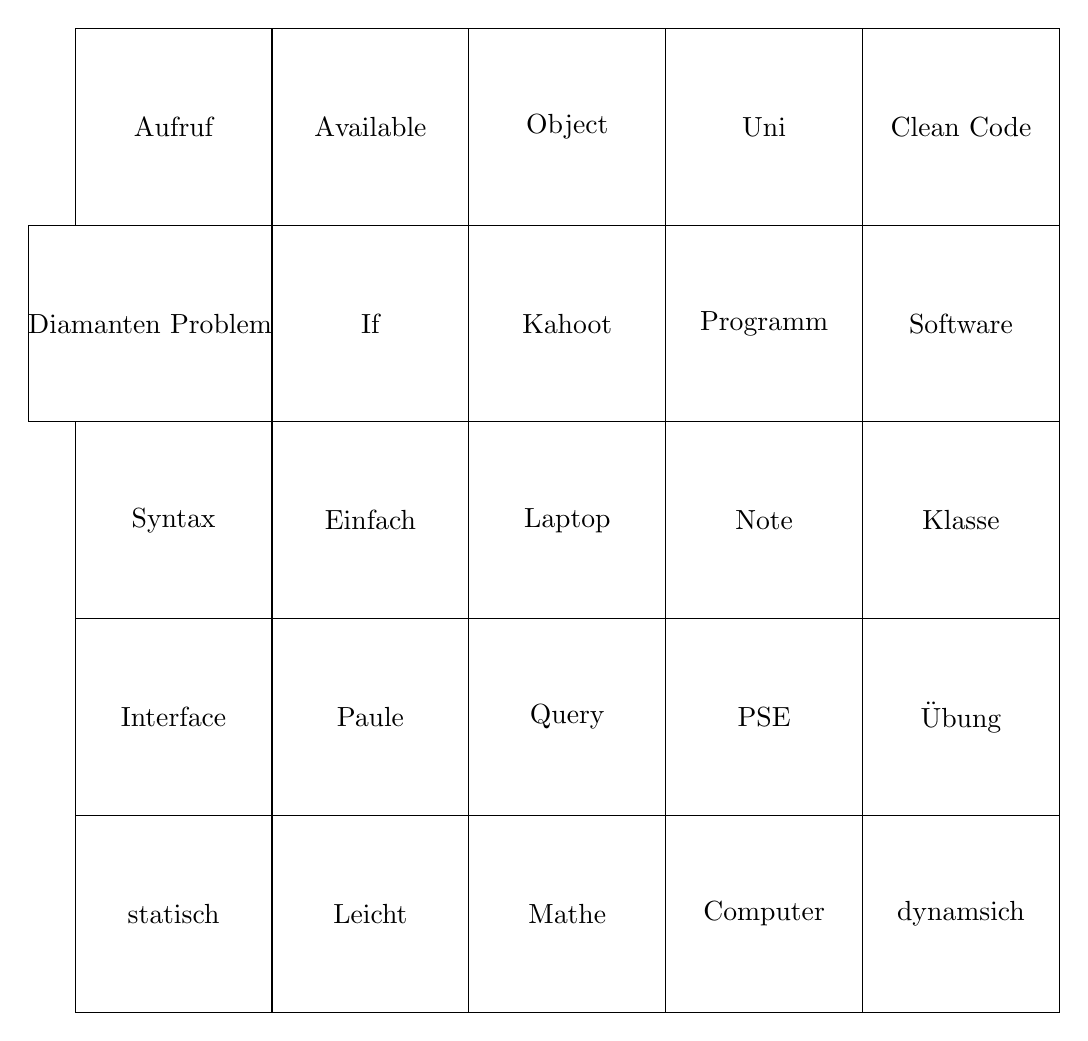
\begin{tikzpicture}[rect/.style={draw, rectangle,anchor=north east, minimum width=\s, minimum height=\s, draw, inner sep=0pt}]
    % First row
    \node[rect] (rect-1-1) at (1*\s,1*\s) {statisch};
    \node[rect] (rect-1-2) at (2*\s,1*\s) {Leicht};
    \node[rect] (rect-1-3) at (3*\s,1*\s) {Mathe};
    \node[rect] (rect-1-4) at (4*\s,1*\s) {Computer};
    \node[rect] (rect-1-5) at (5*\s,1*\s) {dynamsich};

    \node[rect] (rect-1-1) at (1*\s,2*\s) {Interface};
    \node[rect] (rect-1-2) at (2*\s,2*\s) {Paule};
    \node[rect] (rect-1-3) at (3*\s,2*\s) {Query};
    \node[rect] (rect-1-4) at (4*\s,2*\s) {PSE};
    \node[rect] (rect-1-5) at (5*\s,2*\s) {Übung};

    \node[rect] (rect-1-1) at (1*\s,3*\s) {Syntax};
    \node[rect] (rect-1-2) at (2*\s,3*\s) {Einfach};
    \node[rect] (rect-1-3) at (3*\s,3*\s) {Laptop};
    \node[rect] (rect-1-4) at (4*\s,3*\s) {Note};
    \node[rect] (rect-1-5) at (5*\s,3*\s) {Klasse};

    \node[rect] (rect-1-1) at (1*\s,4*\s) {Diamanten Problem};
    \node[rect] (rect-1-2) at (2*\s,4*\s) {If};
    \node[rect] (rect-1-3) at (3*\s,4*\s) {Kahoot};
    \node[rect] (rect-1-4) at (4*\s,4*\s) {Programm};
    \node[rect] (rect-1-5) at (5*\s,4*\s) {Software};

    \node[rect] (rect-1-1) at (1*\s,5*\s) {Aufruf};
    \node[rect] (rect-1-2) at (2*\s,5*\s) {Available};
    \node[rect] (rect-1-3) at (3*\s,5*\s) {Object};
    \node[rect] (rect-1-4) at (4*\s,5*\s) {Uni};
    \node[rect] (rect-1-5) at (5*\s,5*\s) {Clean Code};

\end{tikzpicture}
\newpage
%
% repeated bingo segment (templated)
\section*{PSE BINGO}
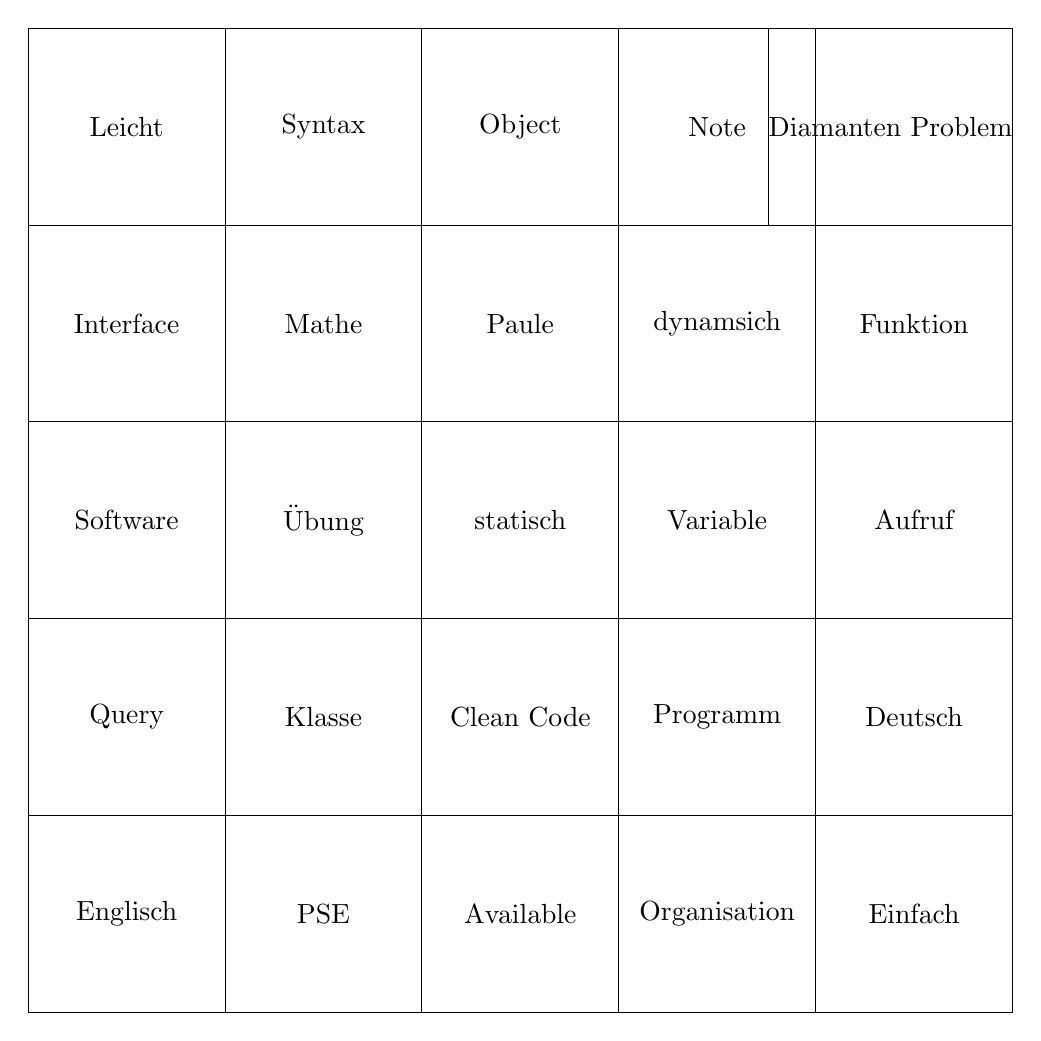
\begin{tikzpicture}[rect/.style={draw, rectangle,anchor=north east, minimum width=\s, minimum height=\s, draw, inner sep=0pt}]
    % First row
    \node[rect] (rect-1-1) at (1*\s,1*\s) {Englisch};
    \node[rect] (rect-1-2) at (2*\s,1*\s) {PSE};
    \node[rect] (rect-1-3) at (3*\s,1*\s) {Available};
    \node[rect] (rect-1-4) at (4*\s,1*\s) {Organisation};
    \node[rect] (rect-1-5) at (5*\s,1*\s) {Einfach};

    \node[rect] (rect-1-1) at (1*\s,2*\s) {Query};
    \node[rect] (rect-1-2) at (2*\s,2*\s) {Klasse};
    \node[rect] (rect-1-3) at (3*\s,2*\s) {Clean Code};
    \node[rect] (rect-1-4) at (4*\s,2*\s) {Programm};
    \node[rect] (rect-1-5) at (5*\s,2*\s) {Deutsch};

    \node[rect] (rect-1-1) at (1*\s,3*\s) {Software};
    \node[rect] (rect-1-2) at (2*\s,3*\s) {Übung};
    \node[rect] (rect-1-3) at (3*\s,3*\s) {statisch};
    \node[rect] (rect-1-4) at (4*\s,3*\s) {Variable};
    \node[rect] (rect-1-5) at (5*\s,3*\s) {Aufruf};

    \node[rect] (rect-1-1) at (1*\s,4*\s) {Interface};
    \node[rect] (rect-1-2) at (2*\s,4*\s) {Mathe};
    \node[rect] (rect-1-3) at (3*\s,4*\s) {Paule};
    \node[rect] (rect-1-4) at (4*\s,4*\s) {dynamsich};
    \node[rect] (rect-1-5) at (5*\s,4*\s) {Funktion};

    \node[rect] (rect-1-1) at (1*\s,5*\s) {Leicht};
    \node[rect] (rect-1-2) at (2*\s,5*\s) {Syntax};
    \node[rect] (rect-1-3) at (3*\s,5*\s) {Object};
    \node[rect] (rect-1-4) at (4*\s,5*\s) {Note};
    \node[rect] (rect-1-5) at (5*\s,5*\s) {Diamanten Problem};

\end{tikzpicture}
\newpage
%
% repeated bingo segment (templated)
\section*{PSE BINGO}
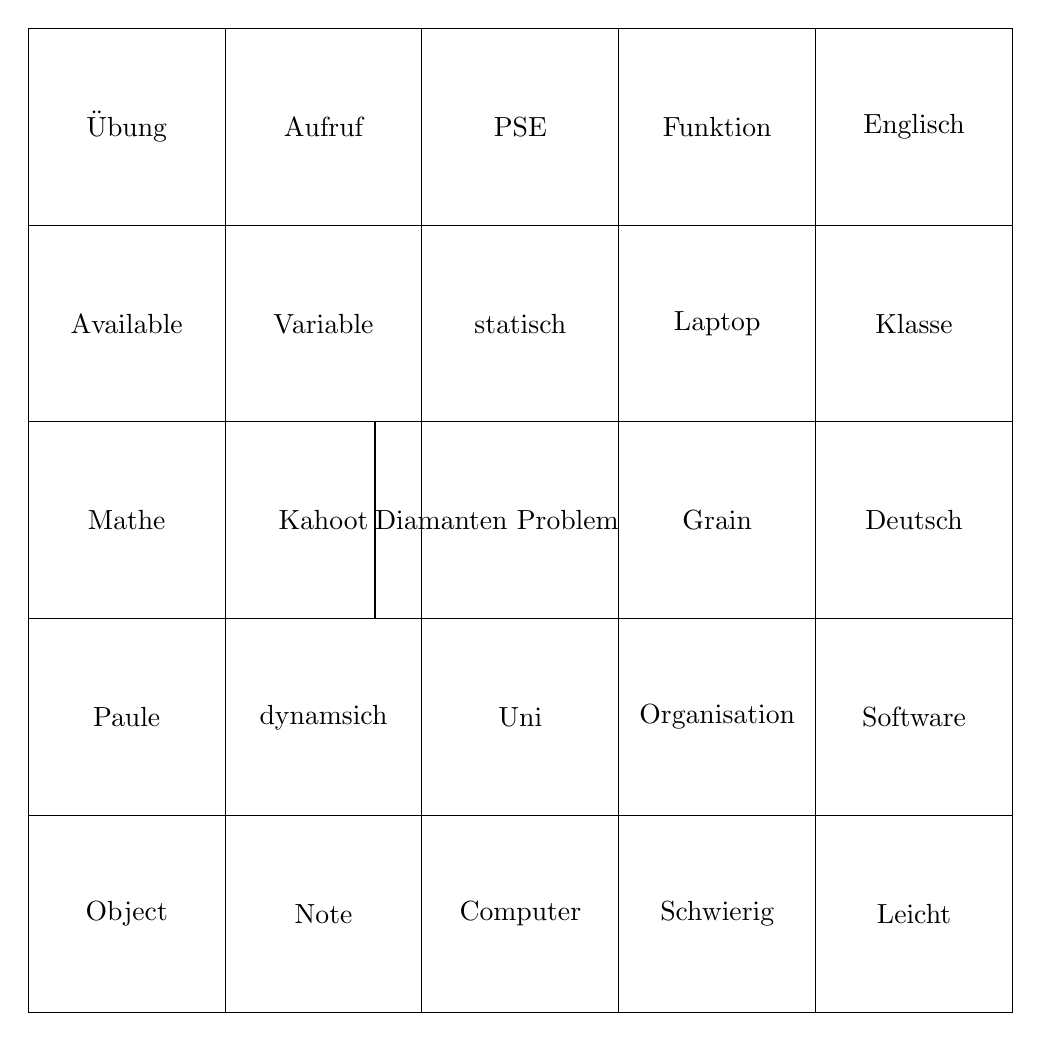
\begin{tikzpicture}[rect/.style={draw, rectangle,anchor=north east, minimum width=\s, minimum height=\s, draw, inner sep=0pt}]
    % First row
    \node[rect] (rect-1-1) at (1*\s,1*\s) {Object};
    \node[rect] (rect-1-2) at (2*\s,1*\s) {Note};
    \node[rect] (rect-1-3) at (3*\s,1*\s) {Computer};
    \node[rect] (rect-1-4) at (4*\s,1*\s) {Schwierig};
    \node[rect] (rect-1-5) at (5*\s,1*\s) {Leicht};

    \node[rect] (rect-1-1) at (1*\s,2*\s) {Paule};
    \node[rect] (rect-1-2) at (2*\s,2*\s) {dynamsich};
    \node[rect] (rect-1-3) at (3*\s,2*\s) {Uni};
    \node[rect] (rect-1-4) at (4*\s,2*\s) {Organisation};
    \node[rect] (rect-1-5) at (5*\s,2*\s) {Software};

    \node[rect] (rect-1-1) at (1*\s,3*\s) {Mathe};
    \node[rect] (rect-1-2) at (2*\s,3*\s) {Kahoot};
    \node[rect] (rect-1-3) at (3*\s,3*\s) {Diamanten Problem};
    \node[rect] (rect-1-4) at (4*\s,3*\s) {Grain};
    \node[rect] (rect-1-5) at (5*\s,3*\s) {Deutsch};

    \node[rect] (rect-1-1) at (1*\s,4*\s) {Available};
    \node[rect] (rect-1-2) at (2*\s,4*\s) {Variable};
    \node[rect] (rect-1-3) at (3*\s,4*\s) {statisch};
    \node[rect] (rect-1-4) at (4*\s,4*\s) {Laptop};
    \node[rect] (rect-1-5) at (5*\s,4*\s) {Klasse};

    \node[rect] (rect-1-1) at (1*\s,5*\s) {Übung};
    \node[rect] (rect-1-2) at (2*\s,5*\s) {Aufruf};
    \node[rect] (rect-1-3) at (3*\s,5*\s) {PSE};
    \node[rect] (rect-1-4) at (4*\s,5*\s) {Funktion};
    \node[rect] (rect-1-5) at (5*\s,5*\s) {Englisch};

\end{tikzpicture}
\newpage
%
% repeated bingo segment (templated)
\section*{PSE BINGO}
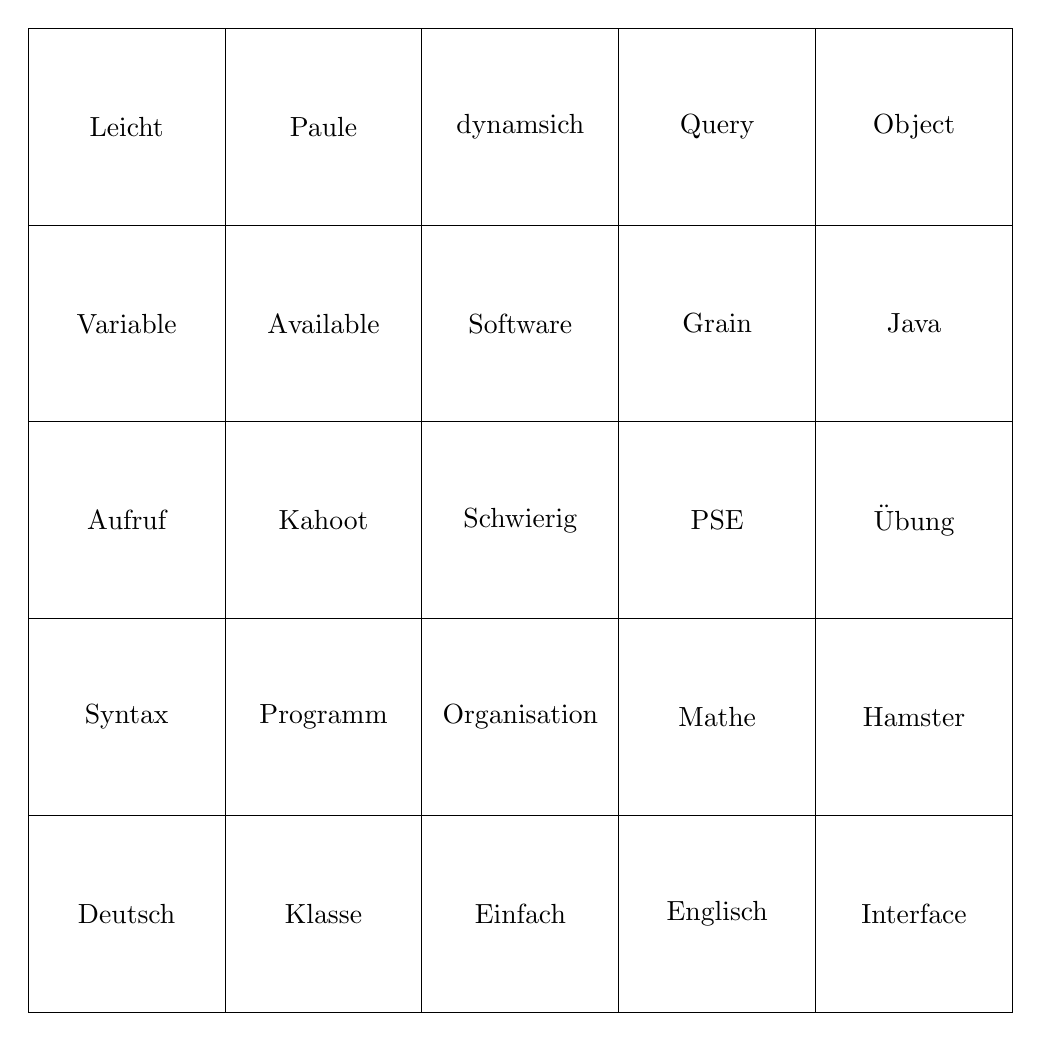
\begin{tikzpicture}[rect/.style={draw, rectangle,anchor=north east, minimum width=\s, minimum height=\s, draw, inner sep=0pt}]
    % First row
    \node[rect] (rect-1-1) at (1*\s,1*\s) {Deutsch};
    \node[rect] (rect-1-2) at (2*\s,1*\s) {Klasse};
    \node[rect] (rect-1-3) at (3*\s,1*\s) {Einfach};
    \node[rect] (rect-1-4) at (4*\s,1*\s) {Englisch};
    \node[rect] (rect-1-5) at (5*\s,1*\s) {Interface};

    \node[rect] (rect-1-1) at (1*\s,2*\s) {Syntax};
    \node[rect] (rect-1-2) at (2*\s,2*\s) {Programm};
    \node[rect] (rect-1-3) at (3*\s,2*\s) {Organisation};
    \node[rect] (rect-1-4) at (4*\s,2*\s) {Mathe};
    \node[rect] (rect-1-5) at (5*\s,2*\s) {Hamster};

    \node[rect] (rect-1-1) at (1*\s,3*\s) {Aufruf};
    \node[rect] (rect-1-2) at (2*\s,3*\s) {Kahoot};
    \node[rect] (rect-1-3) at (3*\s,3*\s) {Schwierig};
    \node[rect] (rect-1-4) at (4*\s,3*\s) {PSE};
    \node[rect] (rect-1-5) at (5*\s,3*\s) {Übung};

    \node[rect] (rect-1-1) at (1*\s,4*\s) {Variable};
    \node[rect] (rect-1-2) at (2*\s,4*\s) {Available};
    \node[rect] (rect-1-3) at (3*\s,4*\s) {Software};
    \node[rect] (rect-1-4) at (4*\s,4*\s) {Grain};
    \node[rect] (rect-1-5) at (5*\s,4*\s) {Java};

    \node[rect] (rect-1-1) at (1*\s,5*\s) {Leicht};
    \node[rect] (rect-1-2) at (2*\s,5*\s) {Paule};
    \node[rect] (rect-1-3) at (3*\s,5*\s) {dynamsich};
    \node[rect] (rect-1-4) at (4*\s,5*\s) {Query};
    \node[rect] (rect-1-5) at (5*\s,5*\s) {Object};

\end{tikzpicture}
\newpage
%

% end not templated
\end{document}